%% MAIN DOCUMENT FOR MASTER THESIS
\documentclass[twoside,english, a4paper, 12pt]{shared/uiofysmaster}
\usepackage[top=1.5in, bottom=1.5in, left=1in, right=1in]{geometry}


% hot to compile in texmaker, sequence:
% pdflatex %.tex | biber % | pdflatex %.tex | evince %.pdf

% le righe importanti
\usepackage[backend=biber,style=numeric,sorting=none]{biblatex}
\addbibresource{bibliography/bibthesis.bib} % qui metti il path del file .bib 

%% TITLE
\author{Lorenzo Speri}
\title{\bf{Analyzing Gravitational Waves through Numerical Simulations of Compact Binaries}}
\date{Supervisor:
Bruno Giacomazzo\\
July 2018}

%% LOAD PACKAGES
\usepackage{listings}
\usepackage{xcolor}
\usepackage{amsmath}
\usepackage{amssymb}
\usepackage{lipsum}
% \usepackage[hidelinks]{hyperref}s
\usepackage{hyperref}
\usepackage{slashed}
\usepackage{simplewick}
\usepackage[squaren]{SIunits}
\usepackage{sidecap}
\usepackage[titletoc]{appendix}
\usepackage{physics}
% units
% \usk is the space
% \per is the division
\usepackage{SIunits}
% tensor
% another possible package
\usepackage{tensind}
\tensordelimiter{:}
%\whenindex{a}{\alpha}{}
%\whenindex{b}{\beta}{}
%\whenindex{g}{\gamma}{}

%% style fo the sections
% format sections
\usepackage{titlesec}
\titleformat{\section}[block]
{\Large\bfseries}
{\thesection}{0.5em}{}


\usepackage{etoolbox}

\usepackage[compat=1.1.0]{tikz-feynman}
\usepackage{multicol}

\patchcmd{\part}{\thispagestyle{plain}}{\thispagestyle{part}}{}{}

\definecolor{grey}{rgb}{0.98,0.98,0.98}
\definecolor{codeRed}{rgb}{0.5, 0.027, 0.02}

% Code parameters
\lstset{language=c++}
\lstset{basicstyle=\small}
\lstset{backgroundcolor=\color{white}}
\lstset{frame=single}
\lstset{stringstyle=\ttfamily}
\lstset{keywordstyle=\color{codeRed}\bfseries}
\lstset{commentstyle=\itshape\color{gray}}
\lstset{showspaces=false}
\lstset{showstringspaces=false}
\lstset{showtabs=false}
\lstset{breaklines}

\setlength{\parskip}{11pt}
\setlength{\parindent}{0mm}

\lstset{
language=Python,
basicstyle=\footnotesize
frame=single,
backgroundcolor=\color{grey}
}

\lstset{
language=Matlab,
basicstyle=\footnotesize,
frame=single,
backgroundcolor=\color{grey}
}

\lstset{
language=C++,
backgroundcolor=\color{grey}
}

\lstdefinelanguage{GLSL}
{
sensitive=true,
morekeywords=[1]{
attribute, const, uniform, varying,
layout, centroid, flat, smooth,
noperspective, break, continue, do,
for, while, switch, case, default, if,
else, in, out, inout, float, int, void,
bool, true, false, invariant, discard,
return, mat2, mat3, mat4, mat2x2, mat2x3,
mat2x4, mat3x2, mat3x3, mat3x4, mat4x2,
mat4x3, mat4x4, vec2, vec3, vec4, ivec2,
ivec3, ivec4, bvec2, bvec3, bvec4, uint,
uvec2, uvec3, uvec4, lowp, mediump, highp,
precision, sampler1D, sampler2D, sampler3D,
samplerCube, sampler1DShadow,
sampler2DShadow, samplerCubeShadow,
sampler1DArray, sampler2DArray,
sampler1DArrayShadow, sampler2DArrayShadow,
isampler1D, isampler2D, isampler3D,
isamplerCube, isampler1DArray,
isampler2DArray, usampler1D, usampler2D,
usampler3D, usamplerCube, usampler1DArray,
usampler2DArray, sampler2DRect,
sampler2DRectShadow, isampler2DRect,
usampler2DRect, samplerBuffer,
isamplerBuffer, usamplerBuffer, sampler2DMS,
isampler2DMS, usampler2DMS,
sampler2DMSArray, isampler2DMSArray,
usampler2DMSArray, struct},
morekeywords=[2]{
radians,degrees,sin,cos,tan,asin,acos,atan,
atan,sinh,cosh,tanh,asinh,acosh,atanh,pow,
exp,log,exp2,log2,sqrt,inversesqrt,abs,sign,
floor,trunc,round,roundEven,ceil,fract,mod,modf,
min,max,clamp,mix,step,smoothstep,isnan,isinf,
floatBitsToInt,floatBitsToUint,intBitsToFloat,
uintBitsToFloat,length,distance,dot,cross,
normalize,faceforward,reflect,refract,
matrixCompMult,outerProduct,transpose,
determinant,inverse,lessThan,lessThanEqual,
greaterThan,greaterThanEqual,equal,notEqual,
any,all,not,textureSize,texture,textureProj,
textureLod,textureOffset,texelFetch,
texelFetchOffset,textureProjOffset,
textureLodOffset,textureProjLod,
textureProjLodOffset,textureGrad,
textureGradOffset,textureProjGrad,
textureProjGradOffset,texture1D,texture1DProj,
texture1DProjLod,texture2D,texture2DProj,
texture2DLod,texture2DProjLod,texture3D,
texture3DProj,texture3DLod,texture3DProjLod,
textureCube,textureCubeLod,shadow1D,shadow2D,
shadow1DProj,shadow2DProj,shadow1DLod,
shadow2DLod,shadow1DProjLod,shadow2DProjLod,
dFdx,dFdy,fwidth,noise1,noise2,noise3,noise4,
EmitVertex,EndPrimitive},
morekeywords=[3]{
gl_VertexID,gl_InstanceID,gl_Position,
gl_PointSize,gl_ClipDistance,gl_PerVertex,
gl_Layer,gl_ClipVertex,gl_FragCoord,
gl_FrontFacing,gl_ClipDistance,gl_FragColor,
gl_FragData,gl_MaxDrawBuffers,gl_FragDepth,
gl_PointCoord,gl_PrimitiveID,
gl_MaxVertexAttribs,gl_MaxVertexUniformComponents,
gl_MaxVaryingFloats,gl_MaxVaryingComponents,
gl_MaxVertexOutputComponents,
gl_MaxGeometryInputComponents,
gl_MaxGeometryOutputComponents,
gl_MaxFragmentInputComponents,
gl_MaxVertexTextureImageUnits,
gl_MaxCombinedTextureImageUnits,
gl_MaxTextureImageUnits,
gl_MaxFragmentUniformComponents,
gl_MaxDrawBuffers,gl_MaxClipDistances,
gl_MaxGeometryTextureImageUnits,
gl_MaxGeometryOutputVertices,
gl_MaxGeometryOutputVertices,
gl_MaxGeometryTotalOutputComponents,
gl_MaxGeometryUniformComponents,
gl_MaxGeometryVaryingComponents,gl_DepthRange},
morecomment=[l]{//},
morecomment=[s]{/*}{*/},
morecomment=[l][keywordstyle4]{\#},
}

% ------------------------------------------------- COLOR BOX

\usepackage{fancyhdr}   
\usepackage{lipsum}

\pagestyle{fancy}
\fancyhead{}% clear headers
\fancyfoot{}% clear footers
\renewcommand{\headrulewidth}{0pt}% eliminate horizontal line
\fancyfoot[RO, LE]{\thepage}







%% MAIN DOCUMENT BEGINNING
\begin{document}

% LOAD COMMANDS
% Equations
\newcommand{\bea}{\setlength{\jot}{10pt}\begin{eqnarray*}}
\newcommand{\eea}{\end{eqnarray*}}
\newcommand{\beq}{\begin{equation}}
\newcommand{\eeq}{\end{equation}}
\newcommand{\bpsi}{\bar{\psi}}
\newcommand{\dslash}{\slashed{\partial}}
\newcommand{\Dslash}{\slashed{D}}
\newcommand{\Lagr}{\mathcal{L}}
\newcommand{\cpp}{\texttt{C++} } 
\newcommand{\mpi}{\texttt{MPI} } 
\newcommand{\de}{\nu}
\newcommand{\T}{\text{TT}}
\maketitle
\clearpage
\thispagestyle{empty}
\tableofcontents
\pagebreak



%% ABSTRACT AND ACKNOWLEDGMENTS
\begin{abstract1}
The observation of gravitational waves marks the beginning of a new era for studying the Universe.
The gravitational radiation plays a crucial role in the theoretical predictions of General Relativity and in the study of violent astrophysical processes, such as compact binary mergers. 
Therefore, we derive the gravitational wave solutions from the Einstein's field equation and we elucidate the implications of the theoretical predictions using different approaches.
Solving the linearized Einstein's field equation, we show that the gravitational radiation produced by a source scales as $1/r$. \\
We present simulations of equal-mass compact binaries with quasi-equilibrium initial conditions.
The gravitational waves produced by black hole binaries with six different quasi-equilibrium initial configurations are studied analyzing the differences between the evolution of the systems.
We investigate the evolution of a binary neutron star system, and we relate the rest mass density evolution to the gravitational wave signal.
We explain the communual characteristics of the gravitational waves of black hole and neutron star binaries, and we briefly explain the differences between the nature of such astronomical objects.
The theoretical prediction, that the angular frequency of the gravitational wave is twice the orbital angular frequency of the rotating binary, is confirmed by the simulations through a Fourier analysis of the gravitational signal.\\
The source code and parameters used for the simulations are publicly available, and they are all based on the open-source Einstein Toolkit code.  
This not only makes it possible to re-run and re-analyze our data, but also enables others to start future researches from this work.
\end{abstract1}
\setcounter{page}{1}


\clearpage
\section{Introduction}
The constancy of the speed of light as measured by observers in different reference frames forces space and time to be mixed into spacetime.
When Albert Einstein developed the General Theory of Relativity, he endowed spacetime with curvature and made it dynamical, creating a theory in which all predictions for physical measurements are invariant under changes in coordinates.
The speed of light is independent of the observer and it is the speed of causality.
Therefore, gravity must be causal as well, and
any change to a gravitating source is communicated to a distant observer no faster than the speed of light $c$.
Such communication of a change in spacetime from a source to an observer leads to the idea that there must exists some notion of gravitational radiation.\\
From the General Theory of Relativity, it is possible to obtain a tensorial wave equation, which governs the behavior of such gravitational radiation.
Therefore, we propose in  section(\ref{from_equation_to_solution}) the derivation of the gravitational wave solution from the Einstein's field equation using the linearized approximation.
Applying the transverse traceless gauge, we find out that the number of radiative degrees of freedom of the general theory of relativity is two.\\
The triumph of theoretical prediction of the gravitational waves (GW) is confirmed by the several experiments.\\
The first indirect evidence of the existence of gravitational waves was given by Hulse and Taylor \cite{weisberg_relativistic_2004,weisberg_timing_2010}. 
From the study of the orbital decay of a binary pulsar, Hulse and Taylor inferred the emission of gravitational waves, since the two neutron stars were spiraling together at just the rate predicted by general relativity’s theory of gravitational radiation reaction.\\
Subsequently, in 2015, the laser interferometer gravitational wave detector LIGO measured directly the signal of a gravitational wave produced by a binary black hole system \cite{abbott_observation_2016}.
And, two years later LIGO-Virgo detector network observed a gravitational-wave signal from the inspiral of two low-mass compact objects consistent with a binary neutron star (BNS) merger \cite{abbott_gw170817:_2017}.\\
So, in order to understand the basic principles of gravitational wave detectors, in section(\ref{effects_gw}) we study how the gravitational waves perturb free falling particles.\\
Then, by studying a ring of free falling test particles, we explain the physical interpretation of the two radiative degrees of freedom two polarization states of the GWs.\\
The gravitational waves are not only the triumph of the General Relativity, but they also give us a completely new method to investigate the nature of binary systems. 
Binary neutron stars and black holes imprint a large amount of information in the produced gravitational radiations.
However, a thorough study of a gravitational signals needs to be combined with accurate numerical simulations of binary mergers in order to fully understand the link between the  gravitational wave production and their sources.\\
So, firstly, we find a simple theoretical model by solving the linearized Einstein's field equation with the presence of matter in section(\ref{production_gw}).
Then, we apply the obtained solution, the so-called quadrupole formula, for a slowly-moving binary source.
And, finally, in the last section(\ref{numerical_evolution}), by using the open-source computational infrastructure Einstein Tookit\cite{loffler_einstein_2012}, we study the relativistic numerical simulations of compact binaries: binary black holes (BBH) with six different quasi-equilibrium initial configurations and a binary neutron star (BNS) is accomplished.
The theoretical prediction from the quadrupole formula, that the frequency of the gravitational wave is twice the orbital angular frequency of the binary, is confirmed in the simulations through a Fourier analysis of the gravitational signal.
In addition, we propose a simple gravitational wave extraction method and we also analyze the rest mass density of the binary neutron stars in order to find the relation with the gravitational signal behavior.\\

\textbf{Notation}\\
Throughout, we will use a spacelike signature $(-,+,+,+)$ and a system of geometrised units in which $G=c=1$, however depending on the need we will also indicate explicitly the speed of light $c=299\,792\,458 \,\metre \per \second$, and the Newton constant of gravitation $G=6.67408 \times 10^{-11} \, \newton \usk \metre^2 \usk \kilogram^{-2}$ \cite{codata_blog_codata_nodate}.\\
We use the Einstein summation convention for  reapeted indexes.
Greek letters are used for summing over all the indeces from 0 up to 3,
whereas latin letters sum only on the spatial indexes 1 2 and 3.\\
We use the controviariant notation of a four-vector
\[
x^{\sigma} = (x^{0},x^{1}, x^{2},x^{3})
\]
or, when we want to aid the comparison with classical Newtonian expression, we use boldface to denote the spatial vectors $\vb{x} =(x,y,z)$ and we rewrite the four-vectors as 
\[
x^{\sigma} = (x^{0},x^{1}, x^{2},x^{3}) = (t,\vb{x}) = (t,x,y,z)
\]
The four-dimensional covariant and partial derivatives will be indicated respectively with $\nabla _{\mu}$ and $\partial _\mu$.\\

\textbf{Codes, Data and Reproducibility of the simulations}\\
The codes used for the numerical simulations, the scripts for the data analysis and the scripts used to generate the figures are available at the website
\\
\url{https://github.com/lorenzsp/thesis}
\\
In addition, we have also included the data produced by the simulations in order to reproduce all the results that we have reported in this paper. \\
In order to reproduce the simulations of the binary black holes and of the binary neutron star, it is possible to download the Einstein Tookit from the website \cite{EinsteinToolkit:web}, and use the parameter files at the website \url{https://github.com/lorenzsp/thesis}.


\clearpage
\section{From the Einstein's Field Equation\\ to Gravitational Wave solutions}
\label{from_equation_to_solution}
Solving the Einstein's field equation is a mathematically complicated problem, because in general it is difficult to find solutions to the field equations which are non-linear    \cite{weinsteinEinsteinDiscoveryGravitational2016}.
Therefore, we will obtain the gravitational wave solutions using the weak field linearized approximation and we will discuss the  gauge transformations that lead to the two radiative degrees of freedom of the Einsten's field equation.\\

\subsection{Linearized Einstein's Field Equation}
The Einstein's field equation is a tensor equation that represents how the geometry of spacetime is related to the presence of masses and energy:
\begin{equation}
\label{einstein_eq}
G_{\mu \nu} \equiv R_{\mu \nu} - \dfrac{1}{2} \,  g_{\mu \nu} \, R =8 \, \pi \, T_{\mu \nu}
\end{equation}
On the right hand side we have the energy-momentum tensor $T_{\mu \nu}$ (or stress-energy tensor), which is interpreted as the flux of four momentum $p^\mu$ accross a surface of constant $x^\nu$. 
On the left hand side the Einstein tensor $G_{\mu \nu}$ includes a measure of the curvature of spacetime through the Ricci tensor $R_{\mu \nu}$, the Ricci scalar $R = R_{\mu \nu} g^{\mu \nu} $ and the metric $g_{\mu \nu}$. \\
In order to solve the Einstein's equation we will make use of the weak field linearized approximation on the metric tensor $g_{\mu \nu}$ and we will derive the Einstein tensor $G_{\mu \nu}$ going through the following steps:
\begin{itemize}

\item[(a)] Calculate the Christoffel symbol
\begin{equation}
\label{christoffel_symbol}
:\Gamma ^\alpha _{\beta \gamma}: = 
\dfrac{1}{2} g^{\alpha \rho} \qty(
\partial_\beta g_{\gamma \rho} + 
\partial_\gamma g_{\rho \beta} -
\partial_\rho g_{\beta \gamma}
)
\end{equation}

\item[(b)] Calculate the Riemann curvature tensor
\begin{equation}
\label{riemann_tensor}
: R^\alpha _{\beta \gamma \sigma}:
=
:\Gamma ^\alpha _{\gamma \lambda}:\,
:\Gamma ^\lambda _{\sigma \beta}:
-
:\Gamma ^\alpha _{\sigma \lambda}:\,
:\Gamma ^\lambda _{\gamma \beta}:
+
\partial_\gamma :\Gamma^\alpha _{\sigma \beta}: 
-
\partial_\sigma :\Gamma^\alpha _{\gamma \beta} :
\end{equation}

\item[(c)] Obtain the Ricci tensor and the Ricci scalar from the Riemann curvature tensor
\begin{equation}
\label{ricci}
R_{\mu \nu} = :R^\alpha _\mu \alpha _\nu: \hspace{1.5cm}
R=\eta^{\mu \nu} R_{\mu \nu} = :R^{\mu} _\mu:
\end{equation}

\end{itemize}

$G_{\mu \nu}$ and $T_{\mu \nu}$ are symmetric tensors, since $g_{\mu \nu}$ is symmetric.
So the Einstein's field equation is a set of non-linear second-order partial differential equations with $10$ linearly independent variables. \\
We show that the equation(\ref{einstein_eq}) leads to gravitational wave solutions if we use the \textbf{weak field linearized approximation}, which means that we treat the spacetime as nearly flat. 
Therefore, we assume the metric tensor $g_{\mu \nu}$ to be equal to the Minkwoski metric $\eta_{\mu \nu}=\text{diag}(-1,+1,+1,+1)$ plus a small metric perturbation $h_{\mu \nu}$ :
\begin{equation}
\label{metric}
g_{\mu \nu} = \eta_{\mu \nu} + h_{\mu \nu}
\end{equation}
where the metric perturbation is symmetric and $\abs{h_{\mu \nu}}\ll 1$ for all $\mu$ and $\nu$. \\
The metric $g_{\mu \nu}$ is also used to lower and raise indeces, however, in linearized theory we consider only the first order approximation in $h_{\mu \nu}$. So, it is possible to raise and lower indeces using the Minkoswkian metric $\eta_{\mu \nu}$.\\ % we can add the estimation of the swarzschild metric the correction at the sun surface h - 10^-6
Taking into account the mentioned approximations, we follow the itemized procedure to derive the so-called linearized Einstein's field equation.\\
The Christoffel symbol is obtained keeping up to the first order in the perturbation $h_{\mu \nu}$
\[
:\Gamma ^\alpha _{\beta \gamma}: = 
\dfrac{1}{2} \eta^{\alpha \rho}
\qty(
\partial_\beta h_{\gamma \rho } 
+
 \partial_\gamma h_{\rho \beta}
-
\partial_\rho h _{\beta \gamma}
) 
\]
Thus, the Riemann curvature tensor becomes 
\setlength{\jot}{10pt}
\begin{eqnarray}
:R^\mu _{\beta \gamma \de }: &=&  \notag
\partial_\gamma :\Gamma ^\mu _{\de \beta}: -
\partial_\de :\Gamma ^\mu _{\gamma \beta}: 
\\ \notag
&=& 
\dfrac{1}{2} 
\qty[
\eta^{\mu \rho} 
\qty(
\partial_\gamma \partial_\de h_{\beta \rho} + %cancel
\partial_\gamma \partial_\beta h_{\de \rho} -
\partial_\gamma \partial_\rho h_{\beta \de}
)
-
\eta^{\mu \sigma} 
\qty(
\partial_\de \partial_\beta h_{\gamma \sigma} +
\partial_\de \partial_\gamma h_{\beta \sigma} - %cancel
\partial_\de \partial_\sigma h_{\beta \gamma}
)
]
\\ 
&=&
\label{reimann_curvature_tensor_first_order}
\dfrac{1}{2} \qty(
\partial_\gamma \partial_\beta :h ^\mu _{\de}: -
\partial_\gamma \partial^\mu h_{\beta \de} -
\partial_\de \partial_\beta :h^\mu _{ \gamma} : +
\partial_\de \partial^\mu h_{\beta \gamma}
)
\end{eqnarray}
where we neglected the first two terms in eq(\ref{riemann_tensor}) because they are second order terms. 
Contracting the first and the third indeces we get the Ricci tensor
\bea
R_{\beta \de} &=& 
\dfrac{1}{2} 
\qty(
\partial_\mu \partial_\beta :h ^\mu _{\de}: -
\partial_\mu \partial^\mu h_{\beta \de} -
\partial_\de \partial_\beta :h^\mu _{\mu } :+ 
\partial_\de \partial^\mu h_{\beta \mu}
) \\
&=&
\dfrac{1}{2} 
\qty(
\partial_\mu \partial_\beta :h^\mu _{\de} : -
\square h_{\beta \de} -
\partial_\de \partial_\beta h +
\partial_\de \partial^\mu h_{\beta \mu}
) 
\eea
where the trace of the perturbation is defined as $h=\eta^{\mu \nu} h_{\mu \nu}= :h^{\mu} _{\mu} :$, and the d'Alambertian opereator in flat space is $\square = \partial_\mu \partial^\mu$. \\
Contracting again to obtain the Ricci scalar yields
\begin{equation*}
\begin{aligned}
R &= \dfrac{1}{2} 
\qty(
\partial_\mu \partial^\nu :h ^\mu _{\nu}: -
\square :h^\beta _{\beta} : -
 \partial_\beta \partial^\beta h +
\partial_\nu \partial^\mu :h^\nu _\mu:
)
\\
&= 
\partial_\mu \partial_\nu h^{\mu \nu} - \square h
\end{aligned}
\end{equation*}
Therefore the Einstein tensor is
\begin{equation}
\label{einstein_tensor_approx}
G_{\beta \nu} = \dfrac{1}{2} 
\qty(
\partial_\mu \partial_\beta :h ^\mu _\nu: -
\square h_{\beta \nu} -
\partial_\nu \partial_\beta h +
\partial_\nu \partial^\mu h_{\beta \mu}
- 
\eta_{\beta \nu} \partial_\mu \partial_\lambda h^{\mu \lambda} - 
\eta_{\beta \nu} \square h
)
\end{equation}
If we define the \textbf{trace-reversed} perturbation metric
\[
\bar{h} _{\mu \nu} = h_{\mu \nu} - \dfrac{1}{2} h \eta_{\mu \nu} \hspace{1.5cm} \bar{h}=\bar{h}^{\mu \nu} \eta_{\mu \nu} = - h
\]
we can simplify the equation(\ref{einstein_tensor_approx}).
Thus,
\begin{equation*}
\begin{aligned}
R_{\beta \nu} &= 
\dfrac{1}{2} 
\qty(
\partial_\mu \partial_\beta \bar{h}^{\mu}\! _{\nu } -
\square \bar{h}_{\beta \nu} -
\cancel{\partial_\nu \partial_\beta h} +
\partial_\nu \partial^\mu \bar{h}_{\beta \mu}
+
\cancel{\dfrac{1}{2} \eta_{\nu \mu} \partial^\mu \partial_\beta h}
-
\dfrac{1}{2} \eta_{\beta \nu} \square h 
+
\cancel{\dfrac{1}{2} \eta_{\beta \mu} \partial_\nu \partial^\mu h}
) \\
&=
\dfrac{1}{2} 
\qty(
\partial_\mu \partial_\beta \bar{h}^{\mu} \!_{\nu } -
\square \bar{h}_{\beta \nu}
+
\partial_\nu \partial^\mu \bar{h}_{\beta \mu}
-
\dfrac{1}{2} \eta_{\beta \nu} \square h 
)
\end{aligned}
\end{equation*}
And contracting the above tensor, we obtain
\begin{equation*}
\begin{aligned}
R &=
\partial_\mu \partial_\beta \bar{h}^{\mu}\! _{\nu } +
 \dfrac{1}{2} \eta^{\mu \nu} \partial_\mu \partial_\nu h - \square h
\end{aligned} = 
\partial_\mu \partial_\nu \bar{h}^{\mu \nu} - 
\dfrac{1}{2} \square h
\end{equation*}
So the Einstein's tensor expressed as a function of $\bar{h} _{\mu \nu}$ is
\begin{equation}
\label{einstein_tensor_tracereversed}
G_{\beta \nu} = \dfrac{1}{2} 
\qty(
\partial_\mu \partial_\beta \bar{h}^\mu \! _{ \nu} -
\square \bar{h}_{\beta \nu}
+
\partial_\nu \partial^\mu \bar{h}_{\beta \mu}
- \eta_{\mu \nu} \partial_\mu \partial_\nu \bar{h}^{\mu \nu}
)
\end{equation}
This expression can be further simplified by choosing an appropriate gauge transformation.
Using the \textbf{Lorenz gauge} condition 
\begin{equation}
\label{lorentz_gauge}
\partial_{\mu} \bar{h}\, ^{\mu \nu} = 0 
\end{equation}
 the Einstein's tensor of equation(\ref{einstein_tensor_tracereversed}) becomes
\bea
G_{\beta \nu} = 
\dfrac{1}{2}
\qty(
\partial_\beta \partial_\mu \bar{h}^{\mu \alpha} \eta_{\alpha \nu}
+ 
\partial_\nu \partial_\mu \bar{h}^{\mu \alpha} \eta_{\alpha \beta}
-
\eta_{\mu \nu} \partial_{\nu} \partial_{\mu} \bar{h}^{\mu \nu}
-
\square \bar{h}_{\beta \nu}
) =
-\dfrac{1}{2} \square \bar{h}_{\beta \nu}
\eea
The linearized Einstein's field equation is
\begin{equation}
\label{linear_einstein_eq}
\square \bar{h}_{\beta \nu} = - 16 \pi\,  T_{\beta \nu} 
\end{equation}
The energy-momentumn tensor $T_{\beta \nu}$ is null in vacuum so the linearized Einstein's equation in vacuum assumes the form of the wave equation in a tensorial form
\begin{equation}
\label{wave_equation}
\square \bar{h}_{\beta \nu} =0  
\end{equation}
The above equation shows that the trace-reversed metric perturbation propagates as a wave distorting a flat spacetime.\\
The simplest solution to the linearized Einstein's equation(\ref{wave_equation}) is a plane wave
\[
\bar{h}_{\beta \nu} = A_{\beta \nu} \, \exp\qty(i\, k_{\alpha} x^{\alpha})
\]
where $A_{\beta \nu}$ is called \textbf{amplitude tensor} and it is symmetric, since $\bar{h}_{\mu \nu}$ is symmetric.\\
Substitution of the plane wave solution into equation(\ref{wave_equation}) implies that $k_{\alpha} k^{\alpha} =0$, so $k^{\alpha}$ is a null four vector. 
Therefore, the plane wave solution is a gravitational wave which travels at the speed of light in the spatial direction $\vb{k} = (k^{1},k^{2},k^{3})/k^{0}$ and with frequency $\omega=k^{0} $, i.e. $\bar{h}_{\beta \nu} = A_{\beta \nu} \, \exp\qty[i\, (\vb{k} \cdot \vb{x} - \omega t)]$.
Furthermore, any $\bar{h}_{\mu \nu}$ satisfying the linearized Einstein's field equation(\ref{wave_equation}) in vacuum describes a \textbf{gravitational wave} propagating at the speed of light, and it can be Fourier-expanded as a superposition of plane waves.\\

\subsection{Gauge Transformations and Radiative Degrees of Freedom}
A \textbf{gauge transformation} in linearized theory is defined as a transformation of the perturbation $h_{\mu \nu}$ into a new metric perturbation $h'_{\mu \nu}$, that satisfies
\begin{equation}
\label{gauge_transf}
h' _{\mu \nu} = h_{\mu \nu} + \partial_\mu \xi _{\nu} + \partial_\nu \xi _{\mu}
\end{equation}
for a given vector field $\xi^\mu$.
Gauge transformations are particularly important because they leave the Riemann curvature tensor unchanged (up to the first order in $h_{\mu \nu}$), such that, the physical spacetime is unchanged (a simple proof can be found in \cite{carroll_spacetime_2003}). 
The invariance of the curvature under such transformations is analogous to the traditional gauge invariance of electromagnetism.\\
Assuming that the Einstein's field equation(\ref{linear_einstein_eq}) are valid everywhere the metric perturbation $h_{\mu \nu}$ contains: gauge degrees of freedom; physical, radiative degrees of freedom; and physical, non-radiative degrees of freedom tied to the matter source of the GW. \\
 It is possible to show that the linearized Einstein's equation can be written as 5 Poisson-type quations, plus a wave equation for the transverse-traceless components of the metric perturbation, which represents the radiative degrees of freedom \cite{flanagan_basics_2005,carroll_spacetime_2003}.\\
 Neverthless this procedure will manifestly demonstrate that the radiative degrees of freedom in spacetime are two, it is a cumbersome and long derivation.
Instead, we neglect the degrees of freedom tied to the matter setting $T_{\mu \nu} =0$ and we analyze only plane wave solutions of equation(\ref{wave_equation}):
\[
\bar{h}_{\mu \nu} = A_{\mu \nu} \, \exp\qty(i\, k_{\alpha} x^{\alpha})
\]
By using the Lorenz gauge and the transverse traceless gauge, we reduce progressively the number degrees of freedom of a plane wave from 10 to 2.\\

We want now to find the conditions on the parameter $\xi_{\mu}$ in order to satisfy the Lorenz gauge condition, that we used in the previous section. 
The initial metric perturbation $h_{\mu \nu}$ tranforms into $h'_{\mu \nu}$ if a gauge transformation is used. However, the new trace reversed metric $\bar{h}'_{\mu \nu}$ transforms as
\begin{eqnarray}
\bar{h}'_{\mu \nu} &=& 
h _{\mu \nu} + 
\partial_\mu \xi _\nu +
\partial_\nu \xi_\mu 
-\dfrac{1}{2} \eta _{\mu \nu}\,
\qty(
 h \, + \partial_\alpha \xi^\alpha +
\partial_\alpha \xi^\alpha  \notag
 )
 \\
 \label{h_bar_gauge}
 \bar{h}'_{\mu \nu} &=&
 \bar{h} _{\mu \nu} + 
\partial_\mu \xi _\nu +
\partial_\nu \xi_\mu 
- \eta _{\mu \nu}\,\partial_\alpha \xi^\alpha 
\end{eqnarray}
Imposing the Lorenz gauge $\partial_{\mu} \bar{h}'\, ^{\mu \nu}=\partial_{\mu} \bar{h}\, ^{\mu \nu} = 0 $ we obtain
\bea
\partial_{\mu} \bar{h}'\, ^{\mu \nu} &=&
\partial_{\mu} \bar{h}\, ^{\mu \nu}+
\partial_{\mu} \partial^\mu \xi ^\nu +
\partial_{\mu} \partial^\nu \xi^\mu -
\partial_{\mu} \eta ^{\mu \nu}\,\partial_\alpha \xi^\alpha 
\\
&=&
0 +
\square \xi^{\nu}+
\partial^\nu \partial_{\mu} \xi^\mu -
\partial^{\nu} \partial_\alpha \xi^\alpha =0
\eea
Any metric perturbation $h_{\mu \nu}$ can therefore be put into a Lorenz gauge by using transformations that satisfy
\[
\square \xi_\mu = 0
\]
The plane wave $\xi_{\mu} = C_{\mu} \exp[i k_{\alpha} x^{\alpha}]$ is a solution of the above equation and it generates a gauge transformation through the four arbitrary constants $C_{\mu}$. \\
The \textbf{Transverse-Traceless (TT) gauge} is the most convinient gauge for the analysis of the gravitational waves, and it is defined for a plane wave by the following conditions:
\begin{itemize}
\item[a)] The Lorenz gauge condition fixes four components of $A_{\mu \nu}$
\[
\partial^{\mu} \bar{h}_{\mu \nu}=A_{\mu \nu} k^{\nu} =0
\]
The amplitude tensor $A_{\mu \nu}$ and the four vector $k^{\mu}$ are orthogonal.

\item[b)] Three components of the aplitude tensor can be eliminated selecting $\xi_{\mu} = C_{\mu} \exp[i k_{\alpha} x^{\alpha}]$ so that $A^{\mu \nu} u_{\mu} =0$ for some chosen four velocity $u_{\mu}$. Three and not four components are fixed, since one further constraint $k^{\mu} A_{\mu \nu} u^{\nu}$ needs to be satisfied.
 
\item[c)] One component of the aplitude tensor can be eliminated selecting $\xi_{\mu} = C_{\mu} \exp[i k_{\alpha} x^{\alpha}]$ so that $A^{\mu} _{\mu} = 0$.

\end{itemize}
This means that we have suffecient freedom to fix the values of 8 components of $A_{\mu \nu}$ from a), b) and c), hence, reducing the number of independent component from 10 to 2 \cite{bishop_extraction_2016}.
Note that $\bar{h} ^{\T} _{\mu \nu}= h^{\T} _{\mu \nu}$ from c).
\\
What does the TT gauge tell us about gravitational radiation ?\\
Let use consider a test a particle at rest with four-velocity $u^{\alpha} = (1,0,0,0)$ in a nearly flat spacetime. If we orient our spatial coordinate axes so that the a plane gravitational wave is travelling in the positive z-direction (equivalentely $x^{3}$ direction) $k^{\sigma} = (\omega, 0 ,0 ,\omega)$ the transverse traceless conditions becomes
\[ \left.
\begin{aligned}
A^{\T}_{\mu 0} \, \omega + A ^{\T}_{\mu 3} \, \omega &= 0 \\
A^{\T}_{0 \nu}  &= 0 \\
A^{\T} _{00} + A^{\T} _{11} +A^{\T} _{22} + A^{\T} _{33} &= 0
\end{aligned}
\;
\right\}
\quad \Rightarrow \quad
\begin{bmatrix}
0 & 0 & 0 & 0 \\
0 & A^{\T} _{11} & A_{12} ^{\T} & 0 \\
0 & A^{\T} _{12} & -A^{\T} _{11} & 0 \\
0 & 0 & 0 & 0 \\
\end{bmatrix}
\]
As a consequence of the transverse traceless gauge  the only non-zero component of the metric perturbation $\bar{h}^{\T}_{\mu \nu}$ are, respectively, the plus ($+$) and the cross ($\times$) polarization of the gravitational wave
\bea
\bar{h}^{\T} _{11} &=& -\bar{h}^{\T} _{22} \equiv h_{+} \\
\bar{h}^{\T} _{12} &=& \bar{h}^{\T} _{21} \equiv h_{\times}  
\eea
So, the plane wave solution in the TT gauge is:
\beq
\label{matrix_h_tt}
\bar{h}^{\T}_{\mu \nu} =
\begin{bmatrix}
0 & 0 & 0 & 0 \\
0 & h_{+} & h_{\times} & 0 \\
0 & h_{\times} & -h_{+} & 0 \\
0 & 0 & 0 & 0 \\
\end{bmatrix}
\eeq
where we express the real part of the solution with $x^{0}=t$ and $x^{3}=z$ as follow
\bea
h_{+} = A^{\T} _{11} \cos \qty(\omega(t-z)) \\
h_{\times} =  A^{\T} _{12} \cos \qty(\omega(t-z))
\eea
$h_{+}$ and $h_{\times}$ are the two independent polarizations of a gravitational wave and they completely characterize the gravitational wave solution. 
We finally found that the radiative degrees of freedom are only two and they are represented by $h_{+}$ and $h_{\times}$. \\

Generally, within any finite vacuum region it is always possible to find a gauge which is locally transverse and traceless \cite{flanagan_basics_2005}, that is, a guage which satisfies the following general conditions
\bea
h_{0 \nu} ^{\T} = 0 \\
\eta ^{\mu \nu} h_{\mu \nu} ^{\T} =0 \\
\partial_{\mu} h^{\mu \nu} _{\T} =0
\eea
The transverse traceless gauge does not only simplify the expression of the perturbation metric, but it also gives an important relation between the Riemann curvature tensor and the metric perturbation.
Since we have already calculated the Riemann curvature tensor in equation(\ref{reimann_curvature_tensor_first_order}) we recall the result taking into account the TT gauge conditions
\begin{eqnarray}
:R^\mu _{00 \sigma }: 
&=&
\dfrac{1}{2} \qty(
\partial_0 \partial_0 :h^{\T \mu} _{\sigma}: -
\partial_0 \partial^\mu h^{\T}_{0 \sigma} -
\partial_\sigma \partial_0 :h^{\T \,\mu} _{ 0}:  +
\partial_\sigma \partial^\mu h_{0 0} ^{\T}
) \notag
\\
&=&
\label{reimann_tensor_TT}
\dfrac{1}{2} \partial_0 \partial_0 :h^{\T \mu} _{\sigma}: 
\hspace{1.5cm} \text{using } h^{\T} _{\mu 0} =0 
\end{eqnarray}
The above result tells us that the curvature of spacetime is proportional to the 'acceleration' of the gravitational wave. 
Considering a plane wave we have
\[
 :R^\mu _{00 \sigma }: = -\dfrac{1}{2} \omega^2 :A^{\T \mu} _{\sigma}: \cos (\omega (t-z))
\]
where $\omega$ is the frequency of the plane wave. 
The curvature is proportional to the square of the frequency, in fact we expect a bigger curvature if the wave oscillates more times per second.
Neverthless we considered the simple model of a plane wave, we can say, naively, that the spacetime is more curved if the ripples of the GW are squeezed in a narrow time interval.
Analogously, the electromagnetic field of an oscillating electric dipole is proportional to the square of the frequency, in fact we expect a more intense  field if the charge oscillates more times per second.




\clearpage
\section{Effects of Gravitational Waves}
\label{effects_gw}
We have shown how the gravitational waves are obtained from the Einstein's field equation. 
By using the transverse traceless gauge we introduced crucial semplifications. 
We want now to explain the important physical consequences of the theoretical results obtained in the previous part.
Throughout the next sections we will use the linearized theory of gravitatinal waves and we consider our metric to be in the TT Gauge.
\subsection{Free particles}
In general relativity the trajectory of a free falling particle is described by the \textbf{geodesic equation}
\begin{equation}
\label{geodesic_eq}
\dv[2]{x^{\beta}}{\tau} + :\Gamma^{\beta} _{\mu \nu}: \,\dv{x^{\mu}}{\tau} \dv{x^{\nu}}{\tau} = 0
\end{equation}
where the coordinates of the particle are represented $x^{\beta}$ and $\tau$ is the proper time.\\
We choose a frame in which a test particle is initially at rest, i.e. with initial four-velocity
\[
u^{\mu} = \dv{x^{\mu}}{\tau} = (1,0,0,0)
\]
We consider a plane wave in the TT gauge propagating towards the test particle. \\
Equation(\ref{geodesic_eq}) can be used to express the initial acceleration of the particle
\[
\qty(
\dv{u^{\beta}}{\tau} 
)_{0}
=
- :\Gamma^{\beta} _{0 0}: 
= -\dfrac{1}{2} \eta ^{\beta \alpha}
\qty(
\partial_{0} h_{\alpha 0} + 
\partial_{0} h_{0 \alpha} + 
\partial_{\alpha} h_{0 0}
)
\]
However, we recall from the TT gauge that
\[
h^{\T}_{0 \alpha} = 0 \qquad  \qquad h^{\T}_{\mu \nu} = \bar{h}^{\T}_{\mu \nu} 
\]
for all $\alpha$. Hence, the initial acceleration of the particle is zero and a free particle, initally at rest, will remain at rest indefinitely.\\
In this constext ''being at rest'' means that the coordinates of the particle do not change, so the TT gauge is a good choice of coordinate. As the gravitational waves propagates, the coordinate system moves with the ripples of the spacetime, in order to keep the particle in the initial position. \\
In the TT gauge free falling bodies are not influenced by  GWs, and their coordinate separation is constant. However, the proper separation is not constant, so let us calculate it.\\
Consider two free falling test particles located at $z=0$ and separated on the x axis by a coordinate distance $L_c$. We still consider a plane wave in the TT gauge propagating in the z direction.\\
The proper distance between the particles is
\bea
L &=& \int _0 ^{L_c} \abs{g_{\mu \nu} \, \dd x^{\mu }\dd x^{\nu }}^{1/2}
=
\int _0 ^{L_c} \sqrt{g_{11}}\dd x = 
\int _0 ^{L_c} \sqrt{1 + h_{+} (t,z=0)} \dd x \\
&\approx &
\int _0 ^{L_c} \qty(1 +\dfrac{1}{2} h_{+} (t,z=0) ) \dd x = L_c \qty(1 + \dfrac{1}{2} h_{+} (t,z=0))
\eea
The proper distance is streched by the passing gravitational wave and the two particles oscillate with a fractional length change given by
\begin{equation}
\dfrac{\delta L}{L} \approx \dfrac{1}{2} h_{+} (t,z=0)
\end{equation}
The proper distance is a very important quantity for a laser interferometer gravitational wave detector, because the phase $\delta \phi$ accumualated by a photon that travels down and back the arm of a laser interferometer is
\[
\delta \phi = \dfrac{4 \pi \delta L}{\lambda}
\]
where $\lambda$ is the wavelength and $\delta L$ is the distance the mirror moves relative to the beam splitter.
Although we used TT gauge to calculate the above formula, it can be shown that this result is gauge independent.\\
If we had considered two particles on the y axis separated by the same coordinate distance, the proper distance would have been
\[
L \approx  L_c \qty(1 - \dfrac{1}{2} h_{+} (t,z=0))
\]
Therefore, recalling the expression of the plus polarization for a plane wave 
$$h_{+} =  A^{\T} _{11} \cos \qty(\omega(t-z))$$ we notice that the particles along x axis are streched, whereas the particles along the y axis are squeezed. 
This is one of the features of the plus polarization, that we will thoroughly analyze in the next section.


\subsection{Geodesic deviation of test particles}
The \textbf{geodesic deviation equation} expresses the relative acceleration between two neighboring geodesics belonging to a one-parameter geodesics $\gamma_s (\tau)$:
\begin{equation}
\label{geudesic_deviation_eq}
\dfrac{D^2}{d \tau ^2} S^{\mu} = :R^{\mu} _{\nu \rho \sigma}: \, T^{\nu} T^{\rho} S^{\sigma}
\end{equation}
 where $S^{\mu} = \partial x^{\mu} / \partial s$ is the deviattion from the geodesic, $T^{\nu} = \partial x^{\mu} / \partial \tau$ is the tangent to the geodesic and the directional covariant derivative is 
\[
\dfrac{D}{d \tau} = \dv{x^{\mu}}{\tau} \, \nabla_{\mu}
\]
The geodesic deviation equation is particularly important because it describes the relative motions of free falling objects and it gives a coordinate-independent measure of the gravitational wave effect. It will also clarify the meaning of the plus and the cross polarizations.\\
If we consider some nearby particles with four-velocities described by a single vector field $u^{\mu}$ and separation vector field $S^{\mu}$, the geodesic deviation equation(\ref{geudesic_deviation_eq}) becomes
\begin{equation}
\dfrac{D^2}{d \tau ^2} S^{\mu} = :R^{\mu} _{\nu \rho \sigma}: \, u^{\nu} u^{\rho} S^{\sigma}
\end{equation}
The four-velocity vector can be approximated with a unit vector in the time direction plus corrections of order $h^{\T} \mu \nu$ and higher, however the Reimann curvature tensor is already first order. Therefore, we ignore the corrections of the four-velocity vector and we write $u^{\nu} =(1,0,0,0)$.\\
Since we have already calculated the Riemann curvature tensor in equation(\ref{reimann_curvature_tensor_first_order}) we recall the result taking into account the TT gauge conditions
\bea
:R^\mu _{00 \sigma }: 
&=&
\dfrac{1}{2} \qty(
\partial_0 \partial_0 :h^{\T \mu} _{\sigma}: -
\partial_0 \partial^\mu h^{\T}_{0 \sigma} -
\partial_\sigma \partial_0 :h^{\T \,\mu} _{ 0}:  +
\partial_\sigma \partial^\mu h_{0 0} ^{\T}
)
\\
&=&
\dfrac{1}{2} \partial_0 \partial_0 :h^{\T \mu} _{\sigma}: \hspace{1.5cm} \text{using } h^{\T} _{\mu 0} =0 
\eea 
In the lowest order approximation the particles are slowly moving, then we have $\tau = x^{0} = t$, so the geodesic deviation equation becomes
\begin{equation}
\pdv[2]{}{t} S^{\mu} = \dfrac{1}{2} S^{\sigma} \pdv[2]{}{t} :h^{\T \mu} _{\sigma}:
\end{equation}
The above equation is a set of differential equations that can be rewritten using the two polarizations of the metric perturbation (equation(\ref{matrix_h_tt}))
\bea
\pdv[2]{}{t} S^{1} &=& \dfrac{1}{2} S^{1} \pdv[2]{}{t} h_{+} + \dfrac{1}{2} S^{2} \pdv[2]{}{t} h_{\times} \\
\pdv[2]{}{t} S^{2} &=& \dfrac{1}{2} S^{1} \pdv[2]{}{t} h_{\times} - \dfrac{1}{2} S^{2} \pdv[2]{}{t} h_{+}
\eea
These can be solved to yield, to lowest order,
\bea
S^{1} = S^{1}(t=0) \qty(1 + \dfrac{1}{2} h_{+})+ \dfrac{1}{2} h_{\times} S^{2}(t=0) \\
S^{2} = S^{2}(t=0) \qty(1 - \dfrac{1}{2} h_{+}) +  \dfrac{1}{2} h_{\times} S^{1}(t=0)
\eea
Let us study the effects of the two polarizations $h_{+}$ and $h_{\times}$ of a gravitational wave, which propagates through the center of a ring of free-falling test particles. 
So, let us use consider a plane wave travelling along the z axis, and let us place a ring of free-falling test particles on the x-y plane  with its center in $(0,0,0)$. 
The ring is initially parametrized by $(\cos \theta, \sin \theta)$ with $\theta \in (0,2\pi]$ and the separation vector $S^{\mu}$ measures the deformation of the ring from its center.\\
Beginning with the case $h_{\times} =0$ and $h_{+} \neq 0$, the solutions of the geodesic deviation equation are
\bea
S^{1} = \cos\theta \qty(1 + \dfrac{1}{2} A^{\T} _{11} \cos (\omega t)) \\
S^{2} = \sin \theta \qty(1 - \dfrac{1}{2} A^{\T} _{11} \cos (\omega t))
\eea
where $h_{+} = A^{\T} _{11} \cos (\omega t)$ for a plane wave. 
The time evolution of the ring is shown in Figure(\ref{plus_polarization}).\\
When the plus polarized gravitational wave propagates through the ring, it increases the proper distance between the ring and its center along the x axis when the phase of the wave is close to $\omega t = 0, 2\pi$, meanwhile it squeezes the test particles along the y axis.
If the phase of the gravitational wave is close to $\omega t = \pi/2, 3\pi/2$ the ring is strecthed along the y axis and the test particles move inwards, therefore, the proper distance from the center of the ring is reduced.
As the wave passes, the test particles bounce back and forth in the shape of $+$ as shown in Figure(\ref{plus_cont}). \\
On the ohter hand, the case where $h_{\times} \neq 0$ and $h_{+} = 0$ yields the geodesic deviation solutions to be
\bea
S^{1} =   \cos \theta + \dfrac{1}{2} \sin \theta A^{\T} _{12} \cos (\omega t) \\
S^{2} = \sin \theta  +  \dfrac{1}{2}  \cos \theta A^{\T} _{12} \cos (\omega t)
\eea
where $h_{\times} = A^{\T} _{12} \cos (\omega t)$ for a plane wave. 
The relationship between these solutions and those for $h_{+} \neq 0$ can be easily found if we consider an angle of $\theta = \pi / 4 $, therefore we obtain
In this case the circle of particles bounce back and forth in the shape of 





\begin{figure}
\centering
    \textbf{ $\mathlarger{\mathlarger{+}}$ Polarization of the gravitational wave}\par\medskip
\makebox[\textwidth][c]{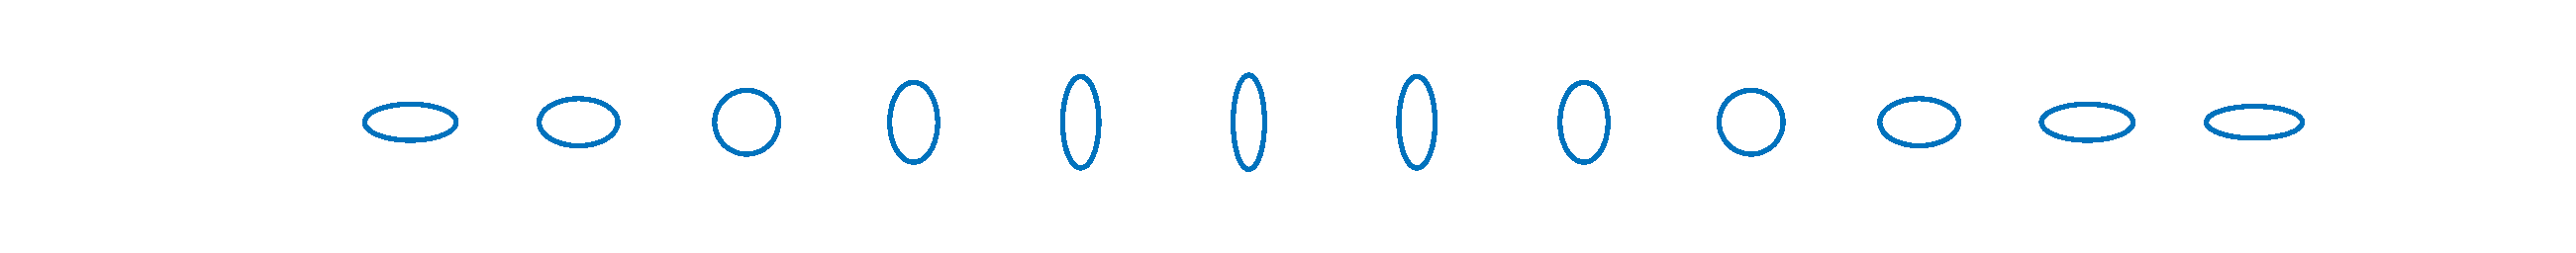
\includegraphics[width=1.3\textwidth]{effects_gw/plus_polarization.eps}}
\caption{Effect of the $h_+$ component on a ring of free-falling test particles at $\omega t = n\pi/6 $ with $n=0,...,12$.}
\label{plus_polarization}
\end{figure}

\begin{figure}
\centering
    \textbf{ $\mathlarger{\mathlarger{\times}}$ Polarization of the gravitational wave}\par\medskip
\makebox[\textwidth][c]{
\includegraphics[width=1.3\textwidth]{effects_gw/times_polarization.eps}}
\caption{Effect of the $h_\times$ component on a ring of free-falling test particles at $\omega t = n\pi/6 $ with $n=0,...,12$.}
\end{figure}

\begin{figure}
\centering
    \textbf{ $\mathlarger{\mathlarger{+}}$ Polarization and $\mathlarger{\mathlarger{\times}}$ Polarization}\par\medskip
\centering
\subfloat[][$+$ polarized gravitational wave.]
   {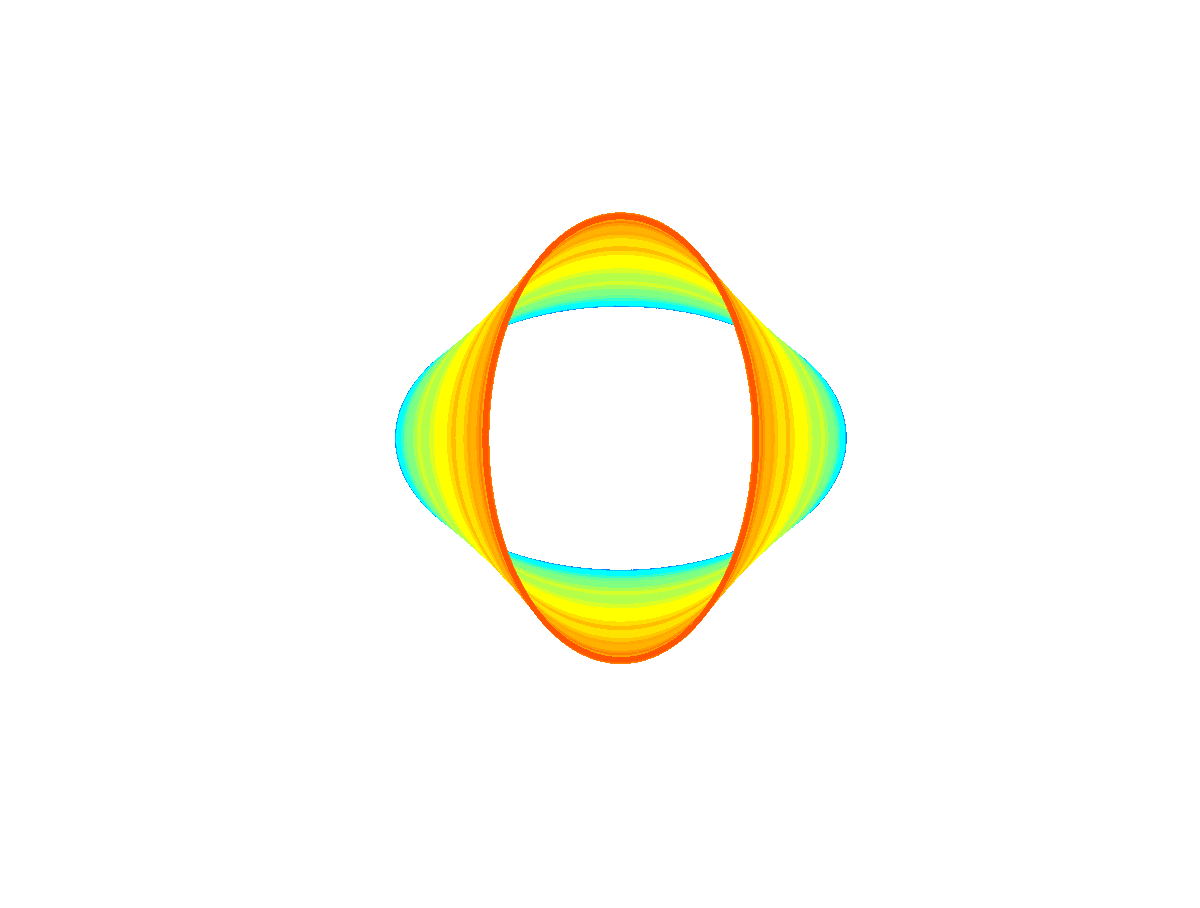
\includegraphics[width=.45\textwidth]{effects_gw/plus_pol_cont.eps}
   \label{plus_cont}} \quad
\subfloat[][$\times$ polarized gravitational wave.]
   {
\includegraphics[width=.45\textwidth]{effects_gw/times_pol_cont.eps}
   \label{times_cont}} \\
\caption{Evolution of a ring of free-falling test particles.}
\label{plus_and_times}
\end{figure}





\subsection{Detection of GW}








\clearpage
\section{Production of Gravitational Waves}
\label{production_gw}
We now want to understand the relation between the gravitational waves and their sources. 
 Therefore,
we make several approximations in order to find a solution of the linearized Einstein's field equation(\ref{linear_einstein_eq}).
In addition, we apply the solution to a slowly moving binary source and we give an estimate of the amplitude of a typical gravitational wave.\\
We will follow a procedure similiar to \cite{carroll_spacetime_2003}, however a derivation of the same result can be found also in \cite{schutz_first_1985,flanagan_basics_2005}.
\subsection{Solution of the Linearized Einstein's Field Equation}
\label{solution_linearized_einstein_eq}
The production of gravitational radiation depends on the movements of objects in spacetime. 
So far, we have neglected the presence of matter and we solved the linearized Einstein's field equation in vacuum. However, if we want to analyze the relation between sources and gravitational waves we need to consider $T_{\mu \nu} \neq 0$ and  solve equation(\ref{linear_einstein_eq}):
\[
\square \bar{h}_{\mu \nu} = - 16 \pi \, T_{\mu \nu}
\]
It is possible to solve this equation using a Green function $G(x^{\sigma} -y^{\sigma})$, such that
\beq
\label{green_equation}
\square_{x} G \qty(x^\sigma - y^{\sigma}) =
\delta^{(4)}  \qty(x^\sigma - y^{\sigma})
\eeq
And the general solution is, then, given by
\begin{eqnarray}
\label{h_green_function}
\bar{h}_{\mu \nu} (x^{\sigma}) =
-16 \pi \int
 G \qty(x^\sigma - y^{\sigma})
 T_{\mu \nu} (y^{\sigma}) 
 \, \dd[4] y 
 \\
 \square_{x} \bar{h}_{\mu \nu} (x^{\sigma}) 
 = 
-16 \pi \int   \square_{x}  G \qty(x^\sigma - y^{\sigma})
 T_{\mu \nu} (y^{\sigma}) 
 \, \dd[4] y 
 =
 - 16 \pi \, T_{\mu \nu} (x^{\sigma})
 \notag
\end{eqnarray}
There are two solutions of equation(\ref{green_equation}): one solution represents a wave travelling forward in time and, the other represents a wave travelling backward in time. 
The two solutions are called, respectively, retarded and advanced. 
We are interested in the \textbf{retarded Green function}, which represents the accumulated effect of signals received at $(x^{0},x^{1},x^{2},x^{3})$ from a source at $(y^{0},y^{1},y^{2},y^{3})$: %mathematical methods in physics
\[
G \qty(x^\sigma - y^{\sigma}) =
-\dfrac{1}{4 \pi\abs{\vb{x} - \vb{y}}} \, \mathlarger{\delta} \qty[\abs{\vb{x} - \vb{y}} - (x^{0}- y^{0})]
\, \theta(x^{0} -y^{0})
\]
where have used boldface to denote the patial vectors $\vb{x} = (x^{1}, x^{2}, x^{3})$ and $\vb{y} =(y^{1}, y^{2}, y^{3})$, with norm $\abs{\vb{x}-\vb{y}} = \qty[\delta_{ij}(x^{i}-y^{i})(x^{j}-y^{j})]^{1/2}$. The Heaviside step function $\theta(x^{0} - y^{0})$ is 1 when $x^{0}>y^{0}$, and zero otherwise. \\
Plugging the retarded Green function into equation(\ref{h_green_function}) and integrating on the $y^{0}$ coordinate we obtain
\beq
\label{h_retarded_solution}
\bar{h}_{\mu \nu} (t,\vb{x}) = 4 \int
\dfrac{1}{\abs{\vb{x}- \vb{y}}} T_{\mu \nu} \qty(t-\abs{\vb{x}-\vb{y}},\vb{y}) \, \dd[3]y 
\eeq
where $t=x^{0}$ and the integration is made over the spatial coordinates. 
From equation(\ref{h_retarded_solution}) we notice that the metric perturbation is influenced by the matter and energy distribution, $T_{\mu \nu}$, at time $t-\abs{\vb{x}-\vb{y}}$. 
Since the gravitational radiation travels at the speed of light $c=1$, the metric perturbation at $(t,\vb{x})$ is influenced by the radiation that was produced by the source at the retarded time $t_r = t-\abs{\vb{x}-\vb{y}}$.\\
We have obtained a general solution, however it possible to derive a more specific formula that will reaveal the quadrupole nature of the gravitational radiation, if we make the following assumptions:
\begin{itemize}
\item \textbf{far field approximation}: the metric perturbation (\ref{h_retarded_solution}) is evaluated at large distances from the source
\begin{equation}
\label{far_field_approx}
\abs{\vb{x}-\vb{y}} \approx \abs{x} \equiv r
\end{equation}
The fractional error of this approximation scales as $\sim L/r$, where $L$ is the size of the source.

\item \textbf{slowly moving source}: the light traverses the source much faster than the components of the cource itself do. Therefore, the source moves at non relativistic speeds.

\item \textbf{isolated system}: the source of the gravitational radiation is an isolated and compact. We assume that our system and the radiation are not gravitationally influenced by other bodies.

\end{itemize}
So we rewrite equation(\ref{h_retarded_solution}) using the far field approximation:
\[
\bar{h}_{\mu \nu} (t,\vb{x}) = \dfrac{4}{r} \int
 T_{\mu \nu} \qty(t-r,\vb{y}) \, \dd[3]y
\]
Since most of the sources are very far from the detection point, the above result is a very good approximation in most of the cases, and it shows the $1/r$ dependency of the gravitational wave.\\
Using the Fourier transform and inverse with respect to time
\bea
\phi (t,\vb{x}) &=&  \mathcal{F}^{-1}[\tilde{\phi}(\omega , \vb{x})] \equiv 
\dfrac{1}{\sqrt{2 \pi}} \, \int \dd \omega e^{-i\omega t} \tilde{\phi}(\omega , \vb{x}) \\
\tilde{\phi} (\omega,\vb{x}) &=&  \mathcal{F}[\phi(t , \vb{x})] \equiv 
\dfrac{1}{\sqrt{2 \pi}} \, \int \dd t e^{i\omega t} \phi (\omega , \vb{x})
\eea
applied to the metric perturbation 
\begin{eqnarray}
\h _{\mu \nu}(\omega , t) 
&\equiv &
\mathcal{F}[\bar{h} _{\mu \nu}(t,\vb{x})]
=
\dfrac{1}{\sqrt{2 \pi}} \, \int  e^{i\omega t} \bar{h}_{\mu \nu} (t , \vb{x}) \; \dd t
\notag
\\
&=&
\dfrac{4}{\sqrt{2 \pi}} \, \int  e^{i\omega t}  \dfrac{T_{\mu \nu}(t_r,\vb{y})}{r} \; \dd t \, \dd ^{3} y
\notag
\\
&=&
\dfrac{4}{\sqrt{2 \pi} \, r} 
\, \int  e^{i\omega (t_r + r)} \, T_{\mu \nu}(t_r,\vb{y}) \; \dd t_r \, \dd ^{3} y
\notag
\\
&=&
\label{F(h)}
\dfrac{4\,  e^{i\omega r}}{r} \int  \, \ten _{\mu \nu}(\omega,\vb{y}) \;  \, \dd ^{3} y
\end{eqnarray}
where we used a change of variable and we defined the Fourier transform of the energy momentum tensor as $\ten _{\mu \nu} \equiv \mathcal{F}[T_{\mu \nu}]$. \\
The Lorenz gauge condition $\partial_{\mu } \bar{h} ^{\mu \nu} =0$ in the Fourier space becomes
\bea
\mathcal{F}\qty[\partial_{0} \bar{h} ^{0 \nu} + \partial_{j} \bar{h} ^{j \nu}] =0
\\
\h ^{0 \nu} = \dfrac{i}{\omega} \partial_{j} \h ^{j \nu}
\eea
As a consequence, we only need to calculate the spacelike components $\h^{j \nu}$.
We set $\nu=k$ in order to find $\h ^{0 k}$ from $\h ^{j k}$, afterwards we use $\h ^{k 0}$ to get $h ^{0 0}$.
The integration by parts of the spacelike components of equation(\ref{F(h)}) is 
\[
\int \ten ^{j k} \dd ^{3} y =
\int \partial_m \qty( \ten ^{m k} y^{j})
\dd ^{3} y
- 
\int \partial_m \qty( \ten ^{m k}) y^{j}
\dd ^{3} y
\]
Since we assumed that the source is isolated, the first term, which is a surface integral, vanishes.
Whereas, the conservation of the energy-momentum tensor $\partial_\mu T^{\mu \nu}=0$ yields in the Fourier space
\[
- \partial_m \qty( \ten ^{m k})  = i \omega \ten ^{0 k}
\] 
Notice that the conservation of the energy-momentum tensor is a very strong assumption, because the motion of bodies is governed by non-gravitational interactions. 
However, and remarkably, the result depends only on the sources motion and not on the forces acting on them \cite{ferrari_quadrupole_nodate}.
Thus,
\bea
\int \ten ^{j k} (\omega , \vb{y}) \dd ^{3} y 
&=&
i \omega \int y^{j} \ten ^{0 k} \; \dd ^{3} y \\
\text{symmetry of } \ten_{k \nu} \rightarrow &=& 
\dfrac{i \omega}{2} \int \qty(
y^{j} \ten ^{0 k} + y^{k} \ten ^{0 j}
) \dd ^{3} y
\\
\partial _l \qty(y^{k} y^{j} \ten ^{0 l}) = \delta ^{k} _{l} y^{j} \ten ^{0l}+
\delta ^{j} _{l} y^{k} \ten ^{0l}+ 
y^{k} y^{j}  \partial _l \ten ^{0 l}
\rightarrow
&=&
\dfrac{i \omega}{2} \int 
\qty[
\partial _l \qty(y^{k} y^{j} \ten ^{0 l})
- 
y^{k} y^{j}  \partial _l \ten ^{0 l}
]
\, \dd ^{3} y
\\
 \partial _l \ten ^{0 l} = \partial _l \ten ^{ l 0} = -i\omega \ten ^{00} \rightarrow &=&
 -
\dfrac{\omega^{2}}{2}
\int
y^{k} y^{j} 
\ten ^{00} (\omega , \vb{y}) \;
\dd ^{3} y
\\
\eea
Then, equation(\ref{F(h)}) becomes
\bea
\h _{k j} &=& 
-\dfrac{4 \, e^{i \omega r}}{r}  
\dfrac{\omega^{2}}{2}
\int
y^{k} y^{j} 
\ten ^{00} (\omega , \vb{y}) \;
\dd ^{3} y
\\
\mathcal{F}\qty[\pdv[2]{T^{00}}{t}] = - \omega ^2 \mathcal{F}[T^{00}]
\rightarrow
&=&
\dfrac{2}{r} \int y^{k} y^{j}
\mathcal{F}\qty[\pdv[2]{}{t}T^{00}(t_r,\vb{y})]
\; 	\dd[3] y 
\\
&=&
\mathcal{F} \qty[\dfrac{2}{r}\, \pdv[2]{}{t} \qty(
 \int
y^{k} y^{j} 
T ^{00} (t_r , \vb{y}) \;
\dd ^{3} y
)
]
\eea
Applying the inverse Fourier-transform to the above result, we obtain the original metric perturbation
\beq
\label{h_bar_quadrupole_formula}
\bar{h}_{kj} = \dfrac{2}{r} \dv[2]{}{t} I_{kj} (t_r)
\eeq
where we define the \textbf{quadrupole moment tensor} 
\begin{equation}
\label{quadrupole_moment_tensor}
I_{k j} (t) =
 \int
y_{k} y_{j} 
T ^{00} (t , \vb{y}) \;
\dd ^{3} y
\end{equation}
To complete the derivation we need to express the metric perturbation in the TT gauge, so we must make the right hand side of equation(\ref{h_bar_quadrupole_formula}) traceless and transverse.\\
We begin by introducing the spatial projection tensor
\begin{equation}
\label{projection_tensor}
P_{i j} = \delta_{i j} - n_{i} n_{j}
\end{equation}
which projects the components of a tensor (with rank 2) into a surface orthogonal to the unit vector $n^{i}$
\[
(P_{i j} X^{i l}) n^{j} = X^{ j l} n_{j}-  n_{i} n_{j} X^{i l} n^{j} = 0
\]
We can use the \textbf{projection tensor} to construct the transverse-traceless version of a symmetric spatial tensor $X_{ij}$ via
\begin{equation}
\label{TT_projection}
X^{TT} _{ij} = \qty(:P_{i}^{k}::P_{j}^{l}: - \dfrac{1}{2} P_{ij} P^{kl}) X_{kl}
\end{equation}
where the first and second terms make the tensor, respectively, transverse and tracless.\\
In addition, we define the \textbf{reduced quadrupole moment tensor} as
\begin{equation}
\label{reduced_quadrupole_moment_tensor}
\mathcal{I}_{kj} = I_{kj} - \dfrac{1}{3} \delta_{kj} I \hspace{1.5cm} \text{where } I=\eta^{ l m} I_{l m} = I^{m} _{m}
\end{equation}
which is traceless, and, for $T^{00} = \rho$, it assume the expression
\[
\mathcal{I} _{kj} = \int \rho(\vb{y}) \qty(y_{k} y_{j} - \dfrac{1}{3}\delta_{kj} y^{l} y_{l} ) \; \dd[3] y
\]
We now have all the concepts to write down 
the \textbf{quadrupole formula}
\begin{equation}
\label{h_TT_quadrupole_formula}
h^{\T}_{ij} = \dfrac{2}{r} \dv[2]{\mathcal{I}_{kl}(t_r)}{t} \qty(:P_{i}^{k}::P_{j}^{l}: - \dfrac{1}{2} P_{ij} P^{kl})
\end{equation}
which represents the metric perturbation of equation(\ref{h_bar_quadrupole_formula}) in the TT gauge, since $h^{\T}_{\mu \nu} = \bar{h} ^{\T}_{\mu \nu}$.\\
Equation(\ref{h_TT_quadrupole_formula}) represents a general solution of the linearized Einstein's field equation, and it shows that the gravitational wave scales as $\sim 1/r$.
\\
The quadrupole formula cannot be used for a black hole because within the Schwarzschild radius of a black hole there is a singularity, which leads to an infinite density.


\subsection{The Nature of the Gravitational Radiation}
The quadrupole formula (\ref{h_TT_quadrupole_formula}) and its derivation gives a  first insight into the properties of the gravitational waves and their sources.\\
Firstly, the gravitational radiation has a \textbf{quadrupolar nature}, because the GW produced by an isolated nonrelativisitc object is proportional to the second derivative of the reduced quadrupole moment of the energy density. \\
We justify qualitatively
the quadrupole nature of the GWs making an anlogy with the electromagnetism.
Let us define the gravitational analogue of the dipole moment: \textbf{mass dipole moment}
\begin{equation}
\label{mass_dipole_moment}
\vb{D} = \sum _{i} m_{i} \vb{x}_i
\end{equation}
where the $m_i$ is the rest mass and $\vb{x}_{i}$ is the spatial postion of particle $i$.\\
In the electromagnetic radiation, the leading contribution to the  comes from the changing dipole moment. 
However, the first derivative of the mass dipole moment is the total linear momentum
\[
\dv{\vb{D}}{t} = \sum _{i} m_i \dv{\vb{x}_i}{t} = \vb{p}
\]
Since the total linear momentum is conserved, there can be no mass dipole radiation from any source.\\
Similiarly, the gravitational analogue of the magnetic dipole moment is 
\[
\vb{\mu} = \sum_{i} \vb{x}_i \times \qty(m_i \dv{\vb{x}_i}{t}) =\vb{J}
\]
where $\vb{J}$ is the total angular momentum of the system. 
Since the total angular momentum is conserved, there can be no dipole radiation of any sort from a gravitational source.
So, the quadrupole moment is the first possible moment which can contribute to the production of GWs.\\

We now study the GW-emission of a binary system in circular orbit with radius $R$.
We assume that two equal-mass stars are orbiting far from each others with an angular frequency $\omega$ and they can be trated as point particles on the $x^{1}-x^{2}$ plane. Thus,
\[
T^{00} (t,\vb{x}) = M \delta(x^{3}) \qty[
\delta\qty(x^{1}-R\cos \omega t)
\delta\qty(x^{2}-R\sin \omega t)
+
\delta\qty(x^{1}+R\cos \omega t)
\delta\qty(x^{2}+R\sin \omega t)
]
\]
The motion of the system is studied using the Newtonian approximations, so using the  Kepler third law we obtain the link between the angular frequency and the radius of the orbit:
\[
\omega ^{2} 
a^{3} = M_T G 
\qquad
\rightarrow
\qquad 
\omega = \qty(\dfrac{M}{4R^{3}})^{1/2}
\]
where we used as total mass of the system $M_T = 2M$, semi-major axis $a=2R$ and $G=1$.\\
The quadrupole moment tensor (\ref{quadrupole_moment_tensor}) becomes
\[
I_{ij}(t) =
2 M R^{2}
\begin{bmatrix}
 \cos ^{2} \omega t  &
 \cos \omega t \sin \omega t &
0
\\
 \cos \omega t \sin \omega t &
 \sin ^{2} \omega t &
0
\\
0 & 0 & 0\\
\end{bmatrix} 
\]
Then, the reduced quadrupole moment (\ref{reduced_quadrupole_moment_tensor}) is easily found to be
\[
\mathcal{I} _{ij}(t) =
2 M R^{2}
\begin{bmatrix}
 \cos ^{2} \omega t -1/3  &
 \cos \omega t \sin \omega t &
0
\\
 \cos \omega t \sin \omega t &
 \sin ^{2} \omega t -1/3&
0
\\
0 & 0 & -1/3\\
\end{bmatrix} 
\]
Taking the second derivative of the above tensor and using the projection tensor with $n_{j} =\delta_{j3} \rightarrow \vb{n} = (0,0,1)$:
\[
P_{jk} = \delta_{jk}- n_{j} n_{k}
\]
we obtain the gravitational wave through the the quadrupole formula(\ref{h_TT_quadrupole_formula}):
\[
h^{\T} _{ij} = \dfrac{8\,G M \,R^{2} \omega^{2}}{c^{4}\, r} \,
\begin{bmatrix}
- \cos 2 \omega t_r   &
 - \sin 2 \omega t_r &
0
\\
  -\sin 2 \omega t_r &
 \cos 2 \omega t_r &
0
\\
0 & 0 & 0\\
\end{bmatrix}
\]
where we inserted $G$ and $c$ in order to give an estimates of the coefficient, and $t_r = t -r/c$ ($r=z$ in this case).\\
Two remarkable aspects of the above formula are that the \textbf{gravitational wave has an angular frequency that is twice the orbital angular frequency at which the system rotates}, and $h_{+} ^{\T}= i h_{\times} ^{\T}$ so the wave is circularly polarized.\\
Let us now give an order-of-magnitude estimate of the amplitude of the gravitational wave, using the coefficient
\[
\mathcal{H} = 
 \dfrac{8\,G M \,R^{2} \omega^{2}}{c^{4}\, r} \,
\]
We assume the two objects to be separated by a distance $R$ equal three times their Schwarzschild radii $r_s=2 G M/c^{2}$.
In addition, if the two objects have approximately the mass of the Sun $M=M_{\odot}=2\times 10^{30} \kilo \gram $ and they rotate with an angular frequency given by the Kepler's third law $\omega = \sqrt{GM/(4R^{3})}$, we have
\bea
\dfrac{G}{c^{4}} \approx 8.26 \times 10^{-45} \kilo \gram^{-1} \, \second ^{2} \meter ^{-1} 
\\
r_s\approx2.95 \times 10^{3} \, \meter
\\
R  = 3 r_s \approx 8.86 \times 10 ^{3} \, \meter
\\
\omega \approx 6.9 \times 10 ^{3} \second ^{-1}
\eea
Pluging into $\mathcal{H}$ and considering the source at the a cosmological distance $r\approx 100 \, \mega pc \approx 3.09 \times 10^{24} \meter$ we have
\[
\mathcal{H} \approx 1.6 \times 10^{-22}
\]
Altough we used Newtonian formulae in a regime where the GR becomes to be important, we obtained a reasonable estimate of the gravitational wave amplitude.\\
Taking into account the discussion we made in section(\ref{free_particles_detection_principles}), if an interferometer of length $L=4 \, \kilo \meter$ was affected by a gravitational wave with intensity $\mathcal{H}$, the strecthing in the arm-length would be of order
\[
\delta L \approx L \, \mathcal{H} \approx 6.38 \times 10^{-19} \, \meter
\]
and the laser light with wavelength $\lambda=10^{-6} \meter$ would acquire a phase shift
\[
\delta \phi = 100 \dfrac{4 \pi}{\lambda} \delta L\approx 8.02 \times 10 ^{-10}
\]


\clearpage
\section{Numerical Evolution of Compact Binaries}
\label{numerical_evolution}

In the linearized approximation, where gravitational fields are weak and velocities are nonrelativistic, we showed that it is straightforward to derive a relationship between the matter dynamics and the emission of gravitational waves, thus obtaining the quadrupole formula.
However, the strongest gravitational-wave signals come from highly compact systems that evolve at relativistic speeds, where the linearized assumptions do not apply. 
Therefore, gravitational-wave detectors find more likely an event which has a powreful signals.
Thus, it is important to be able to calculate gravitational-wave emission accurately for processes such as black hole or neutron star inspiral and merger.
Such problems cannot be solved analytically and instead are modeled by numerical relativity to compute the gravitational field near the source.\\
In this section we study the gravitational-wave signals obtained from numerical simulations of compact binaries, using the Einstein Toolkit, an open-source computational infrastructure for numerical relativity based on Cactus Framework.\\
The Cactus framework [ref] is a general framework for the development of portable, modular applications, wherein programs are split into components (called thorns) with clearly defined dependencies and interactions. 
Thorns are typically developed independently and do not directly interact with each other. 
Cactus simulations require an executable to be compiled, and this executable has one mandatory argument: a parameter file.
The parameter file is a simple text file, containing the desired settings within the simulation, it is used not only to set up the initial conditions and the necessary thorns for the simulation, but also to choose outputs and their format.
\\
A thorough description of the numerical methods used to perform the simulations can be found here, we depict the initial conditions of our simulations and we briefly mention the used thorns.
Rather than analyzing the algorithms of th Einstein Toolkit, the purpose of the following sections is to study the gravitational-wave signals of binaries black holes (BBH) and neutron stars (BNS). 
\subsection{Gravitational Wave Extraction}
\label{gw_extraction}
Using \texttt{WeylScal4}, the Einstein Toolkit calculates the  Newman-Penrose scalar $\psi_4$ [REF], which is linked to the GW strain by the following relation, valid only at spatial infinity:
\begin{equation}
\label{psi_4_strain}
\psi_{4} = \pdv[2]{}{t} \qty(h_{+} - i h_{\times})
\end{equation}
In order for equation(\ref{psi_4_strain}) to be valid, the signal has to be extracted as furthest as possible from the source.
The signal is then decomposed in spin-weighted spherical harmonics of spin $ - 2$ by the thorn \texttt{Multipole} [% K. S. Thorne, Rev. Mod. Phys. 52, 299 (1980). Multipole expansions of gravitational radiation
] 
\[
\psi_4 (t',r,\theta,\phi)= \sum_{l=2} ^{\infty} \, \sum _{m=-l} ^{l=2} \psi^{lm} _4 (t',r) \, _{-2} Y _{lm} (\theta, \phi) 
\]
The output given by the Einstein Toolkit is therefore $\psi_{4} ^{lm} (t',r)$, however, in this work we only focus on the dominant $l = m = 2$ mode and we get the GW strain form following a procedure similiar to REF%modeling equal and un
%mergers
Since $\psi^{lm} _4 (t',r)$ is extracted at a distance $r$ from the source center,  our data detect the signal at a time $t'$, which is different from the instant when the radiation was emitted.
So, we subtract from the output time $t'$ the distance from the source $r$
in order to compute the gravitational radiation as if the signal would have been emitted at the coordinate origin.\\
We are interested in the behavior of the gravitational wave at a given time and distance $(t,r) = (t'-r,r)$, so we neglect the numerical factor $_{-2} Y _{lm} (\theta, \phi)$ given by choosing an arbitrary angle $(\theta,\phi)$ for the spin-weighted spherical harmonics.
Thus, we integrate twice in time in order to get the complex-valued gravitational strain
\[
\tilde{h}(t) = \int _0 ^{t} \int _0 ^{\hat{t}} \psi_4 ^{2,2} (t^{*},r)
\, \dd t^{*} \,  \dd \hat{t}
\]
where we used the trapezodail rule for the numeric integration.
The resulting quantity obtained with the procedure described above show a left-over non-linear drift, which can be eliminated  performing a fit to a second order polynomial for both the real and the imaginary parts of $\tilde{h}(t)$.
The two polarizations (plus and times) of the gravitational wave are finally obtained subtracting the noise
\begin{eqnarray}
\label{h_+_numerical}
h_{+} (t)= \Re {\tilde{h}} -  \qty(Q_0 ^{R} + Q_1 ^{R} t + Q_2 ^{R} t^{2}) \\
\label{h_x_numerical}
h_{\times}(t) = - \qty[
\Im {\tilde{h}} -
\qty(Q_0 ^{I} + Q_1 ^{I} t + Q_2 ^{I} t^{2})
]
\end{eqnarray}
where the $Q$ values are the coefficients of the fitted polynomials for the real $Q^{R}$ and the imaginary $Q^{I}$ parts of $\tilde{h}(t)$.\\

\subsection{Binary Black Hole}
As we have done so far and following the Einstein Tookit conventions, we set $G=c=1$, and therefore we express time and space in units of solar masses $M_{\odot}$, i.e. $1 t [M_{\odot}] \approx 0.005 \milli \second$ and $1 x [M_{\odot}] \approx 1.5 \kilo \meter$.\\
We simulate the evolution of equal-mass binary black holes with different quasi-equilirbium initial conditions.
The thorn \texttt{TwoPunctures} is used to set up the initial data for the two black holes located at the x-axis with opposite linear momentum along the y-axis.
Due to the symmetry of the problem, it is possible to reduce the computational cost by a factor of 2 by not evolving the domain with $z < 0$, and by another factor 2 evolving points with $x > 0$ and populating the missing part by rotating the existing domain for 180 degrees along the z-axis.
An example of initial data set in the parameter file is
\linebreak
\texttt{\\
TwoPunctures::par\_b             =  3.0 \\
TwoPunctures::par\_m\_plus        =  0.47656 \\
TwoPunctures::par\_m\_minus       =  0.47656 \\
TwoPunctures::par\_P\_plus [1]    = +0.13808 \\
TwoPunctures::par\_P\_minus[1]    = -0.13808
\\
}
\linebreak
We call parameter $b$ the parameter \texttt{par\_b} which defines the initial distance of the two black holes at $(x,y,z) = (\pm 3,0,0)$ from the origin of the axes. 
\texttt{par\_m\_plus} and \texttt{par\_m\_minus} set the "bare mass" parameter, and \texttt{par\_P\_plus[1]} and \texttt{par\_P\_minus[1]} set the Bowen-York linear momentum parameter.
We let evolve the binary black hole using six different quasi-equilibrium initial conditions, as shown in Table(\ref{initial_conditions_bbh}).
%%
%%
%%
%%
\begin{table}
\centering
\begin{tabular}{|c|c|c|c|}
\hline 
simulation name & \texttt{par\_b} & \texttt{par\_m\_plus} & \texttt{par\_P\_plus[1]} \\ 
\hline 
BBH-b3 & 3 & 0.47656
 & +0.13808 \\ 
%\hline 
BBH-b4 & 4 & 0.48243 & +0.11148 \\ 
%\hline 
BBH-b5 & 5 & 0.48595 & +0.095433 \\ 
%\hline 
BBH-b6 & 6 & 0.48830 & +0.084541 \\ 
%\hline 
BBH-b7 & 7 &  0.48997 & +0.076578 \\ 
%\hline 
BBH-b10 & 10 & 0.49299 & +0.061542 \\ 
\hline 
\end{tabular} 
\caption{The table shows the quasi-equilibrium initial conditions used in the \texttt{TwoPuncture} thorn. Since the two balck holes have equal masses \texttt{par\_m\_plus}$=$\texttt{par\_m\_minus} and opposite momentum \texttt{par\_P\_plus[1]}$=- $\texttt{par\_P\_minus[1]}, we do not report in the table the obvious initial conditions of the second black hole.}
\label{initial_conditions_bbh}
\end{table}
%%
%%
%%
%%
Each initial configuration is then evolved using the \texttt{ML\_BSSN} (\texttt{McLachlan} BSSN) thorn, the gravitational wave information is extracted using \texttt{WeylScal4} thorn.\\
The orbits of covered by the binaries black hole are shown in Figure(\ref{orbits}).
%%
%%
%%
%%
\begin{figure}
\centering
    \textbf{Orbits of different  configurations of BBH}\par\medskip
\centering
\subfloat[][Trajectory of the BBH with initial distance from the origin $b=3 \, M_{\odot}$.]
   {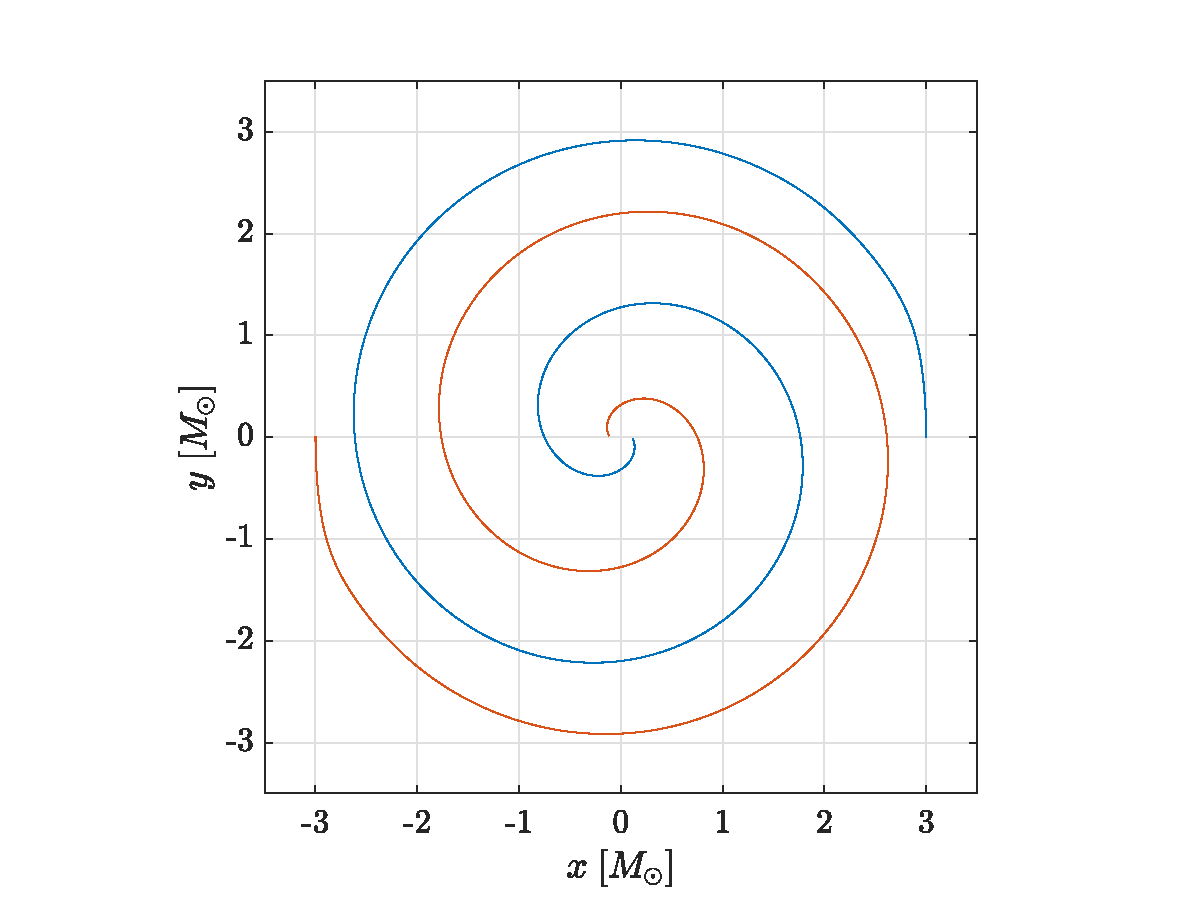
\includegraphics[width=.45\textwidth]{numerical_evolution/trajectory_b3.eps}
   \label{trajectory_b3}} \quad
   \subfloat[][Trajectory of the BBH with initial distance from the origin $b=4 \, M_{\odot}$.]
   {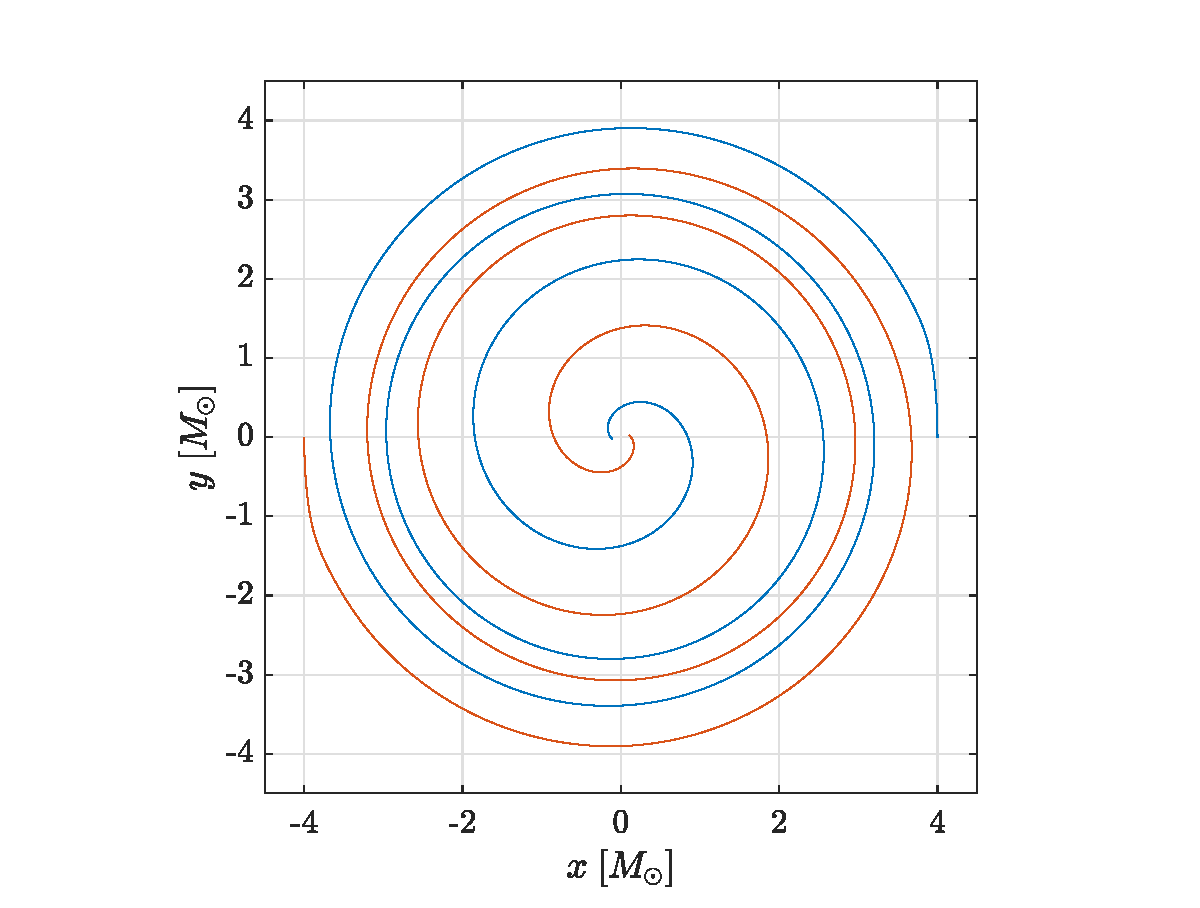
\includegraphics[width=.45\textwidth]{numerical_evolution/trajectory_b4.eps}
   \label{trajectory_b4}} \quad
\subfloat[][Trajectory of the BBH with initial distance from the origin $b=5 \, M_{\odot}$.]
   {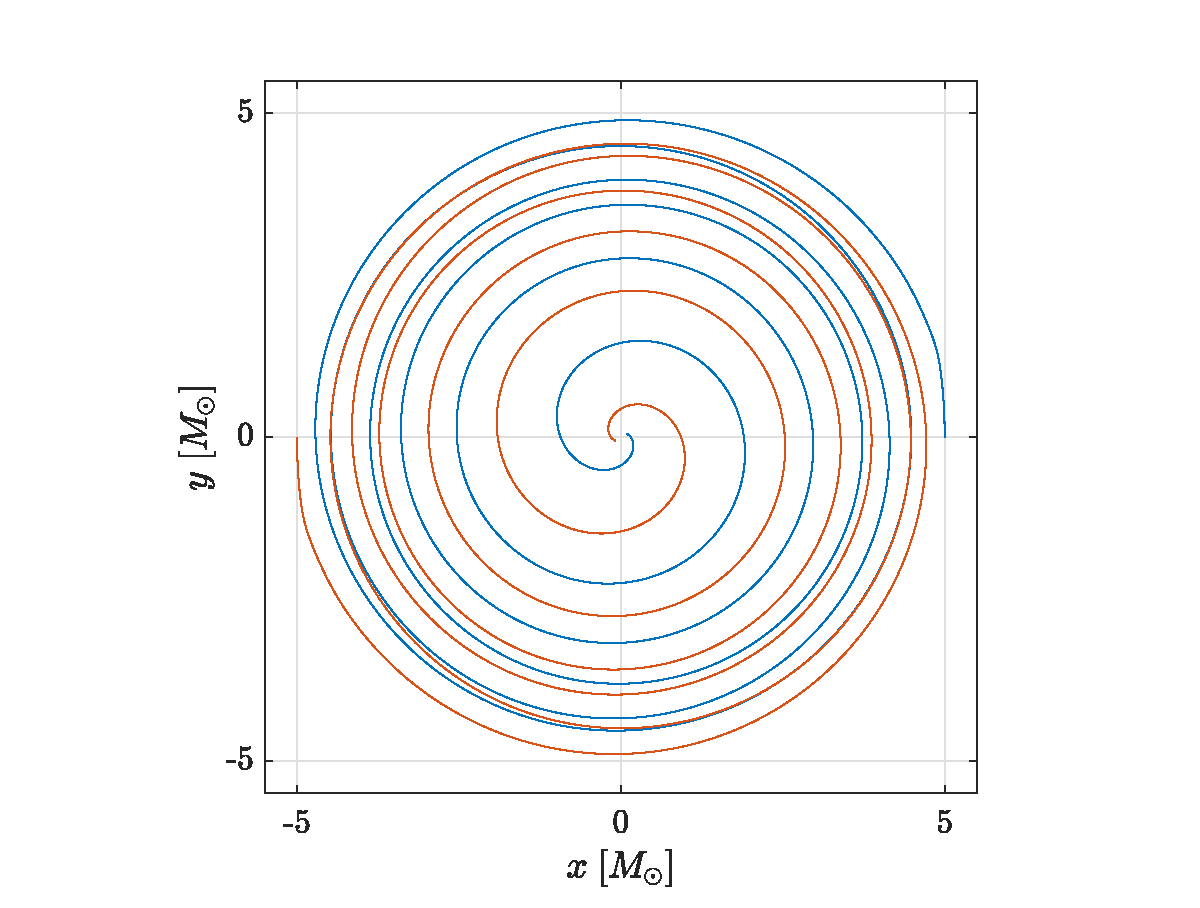
\includegraphics[width=.45\textwidth]{numerical_evolution/trajectory_b5.eps}
   \label{trajectory_b5}} \quad
\subfloat[][Trajectory of the BBH with initial distance from the origin $b=6 \, M_{\odot}$.]
   {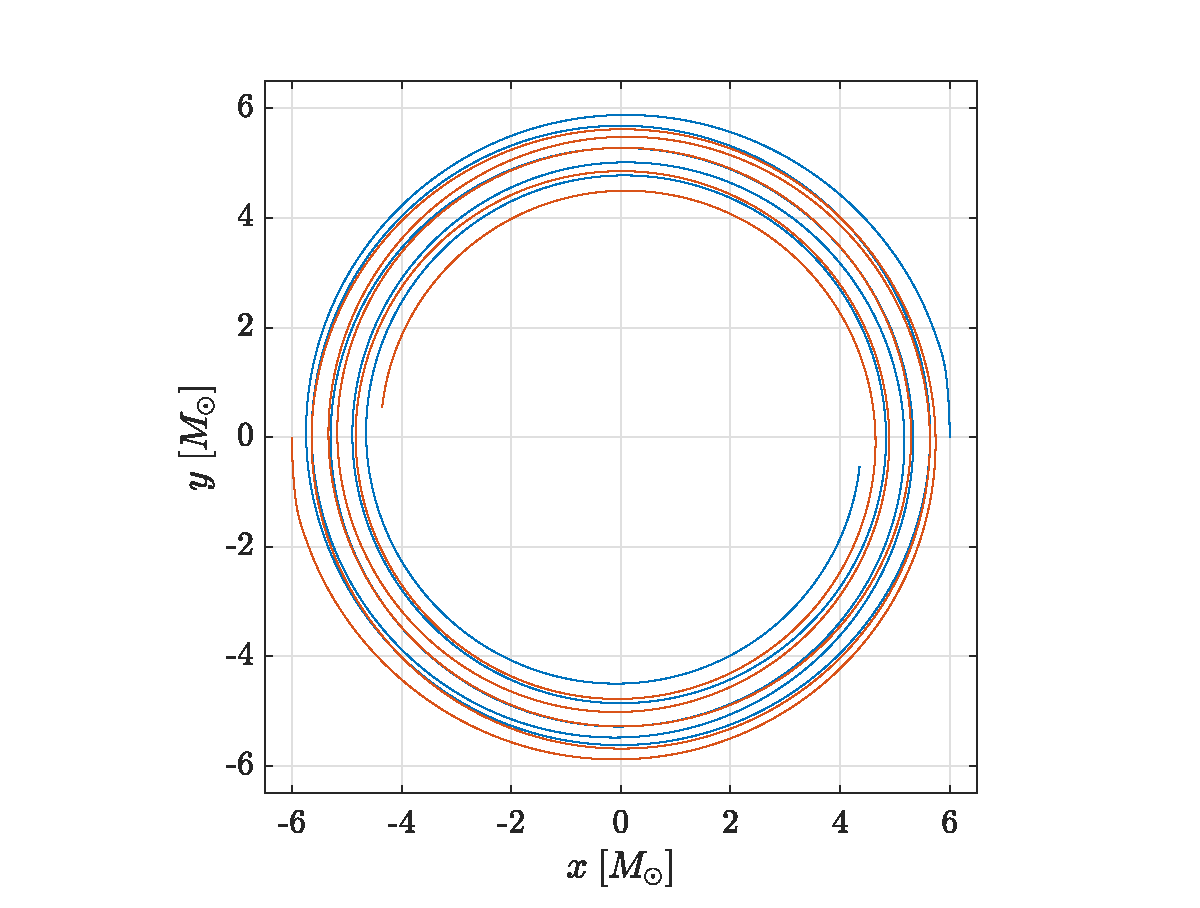
\includegraphics[width=.45\textwidth]{numerical_evolution/trajectory_b6.eps}
   \label{trajectory_b6}} \quad
\subfloat[][Trajectory of the BBH with initial distance from the origin $b=7 \, M_{\odot}$.]
   {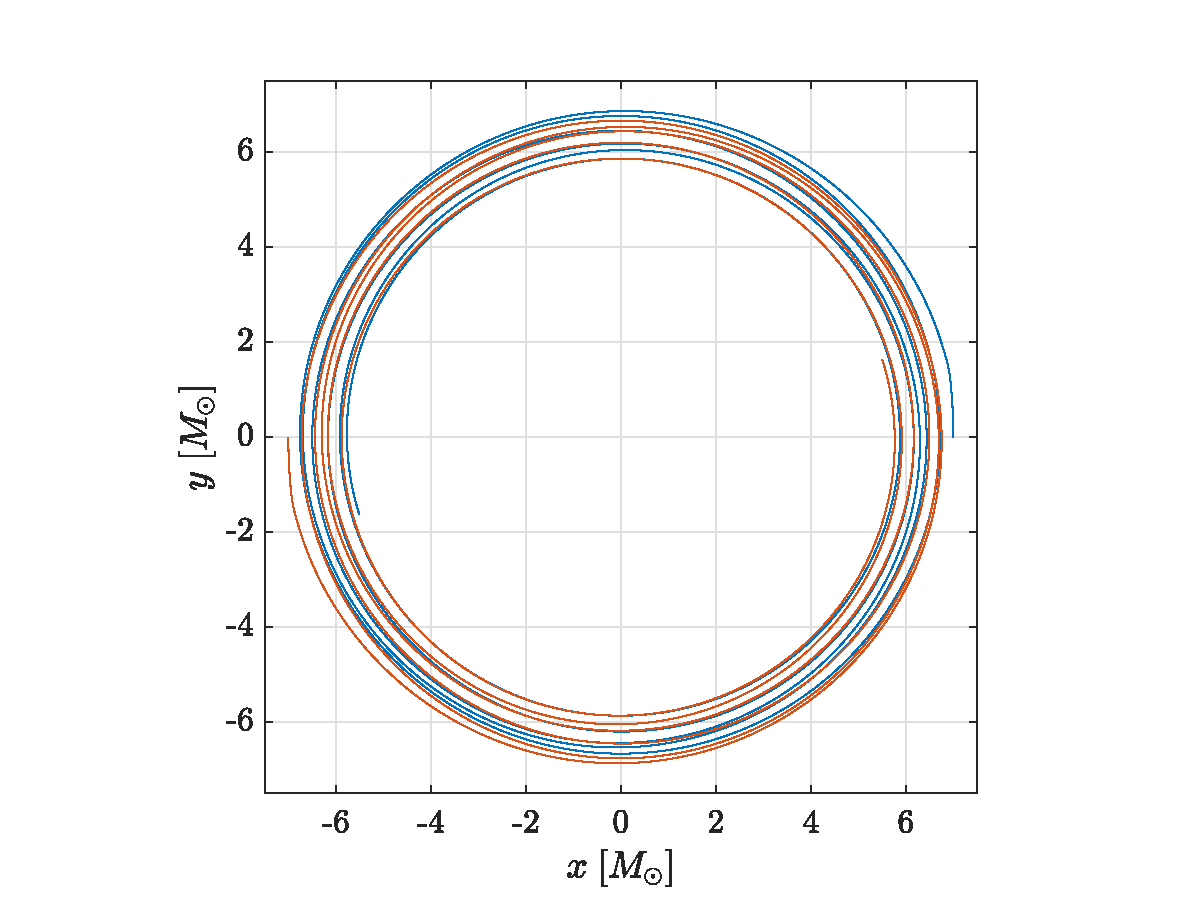
\includegraphics[width=.45\textwidth]{numerical_evolution/trajectory_b7.eps}
   \label{trajectory_b7}} \quad
\subfloat[][Trajectory of the BBH with initial distance from the origin $b=10 \, M_{\odot}$.]
   {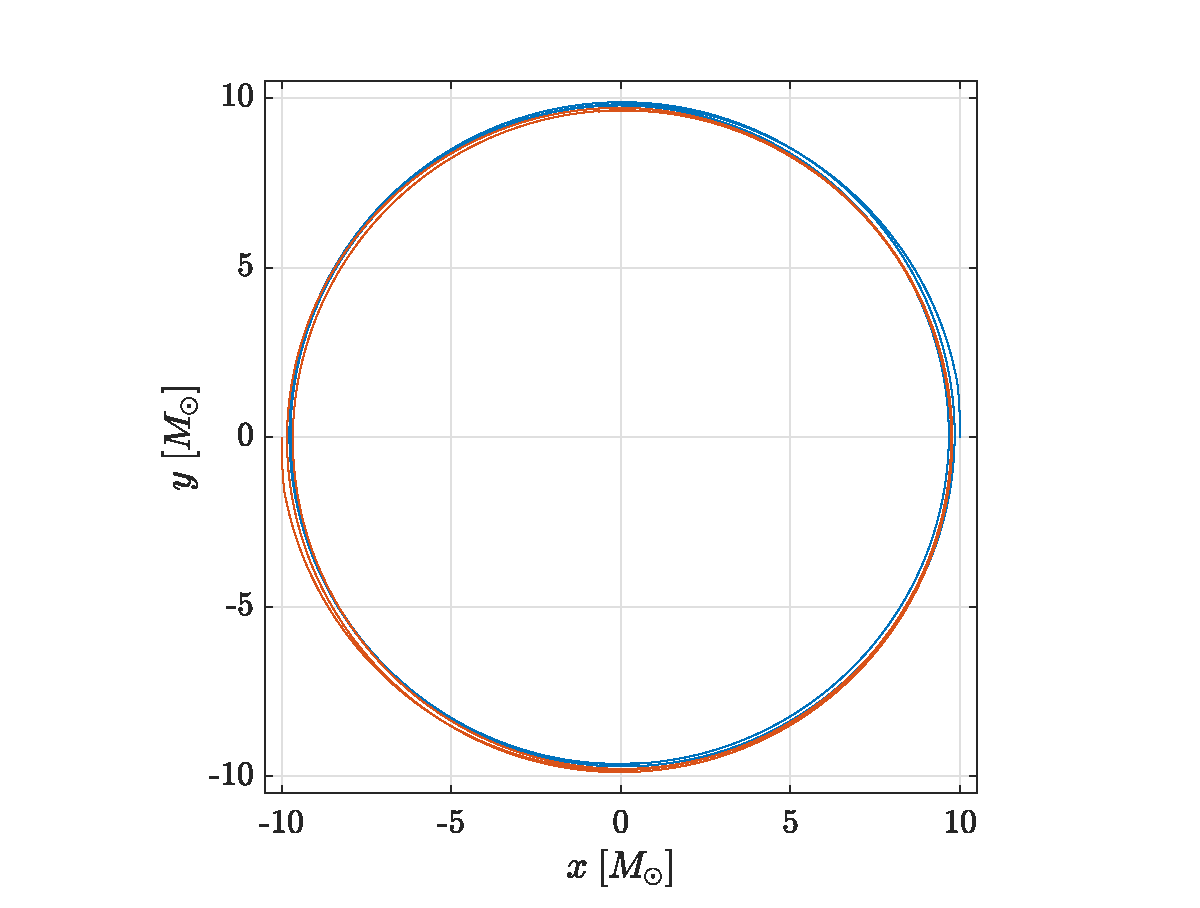
\includegraphics[width=.45\textwidth]{numerical_evolution/trajectory_b10.eps}
   \label{trajectory_b10}} \quad
 \\
\caption{It is shown the evolution of the BBH using the quasi-equilibrium initial conditions of Table(\ref{initial_conditions_bbh}). As the parameter $b$ increases, the orbits of the BBH tend to be more stable, where with stable we mean that the difference between the previous and the next orbit is small.}
\label{orbits}
\end{figure}
%%
%%
%%
%%
Due to the short initial distance from the origin, the BBHs with a  with low $b$ merge after few revolutions, for instance BBH-b3 merges after $2$ revolutions; BBH-b4 merges after
$3.5$ revolutions; BBH-b5 merges after $6$ revolutions.
Whereas the BBHs with an high parameter$b$ have orbits close to each other, such that they form a ring shape.\\
Notice that as the $b$ increases, the two black holes have orbits that drift apart from the coil-shaped path of Figure(\ref{trajectory_b3}).
This behavior can be better understood analyzing the distance of one of the balck hole from the origin as a function of time. 
For this reason, we plot in Figure(\ref{radius_evolution}) the normalized radial distance
\[
R(t)/b = \frac{\sqrt{x ^{2} (t) + y^{2} (t)}}{b}
\]
which depicts a new feature of the orbits. There are evident oscillations of the time-evolution of the radius $R(t)$.
%%
%%
%%
%%
\begin{figure}
\centering
    \textbf{Normalized Radial evolution of the BBH}\par\medskip
\makebox[\textwidth][c]{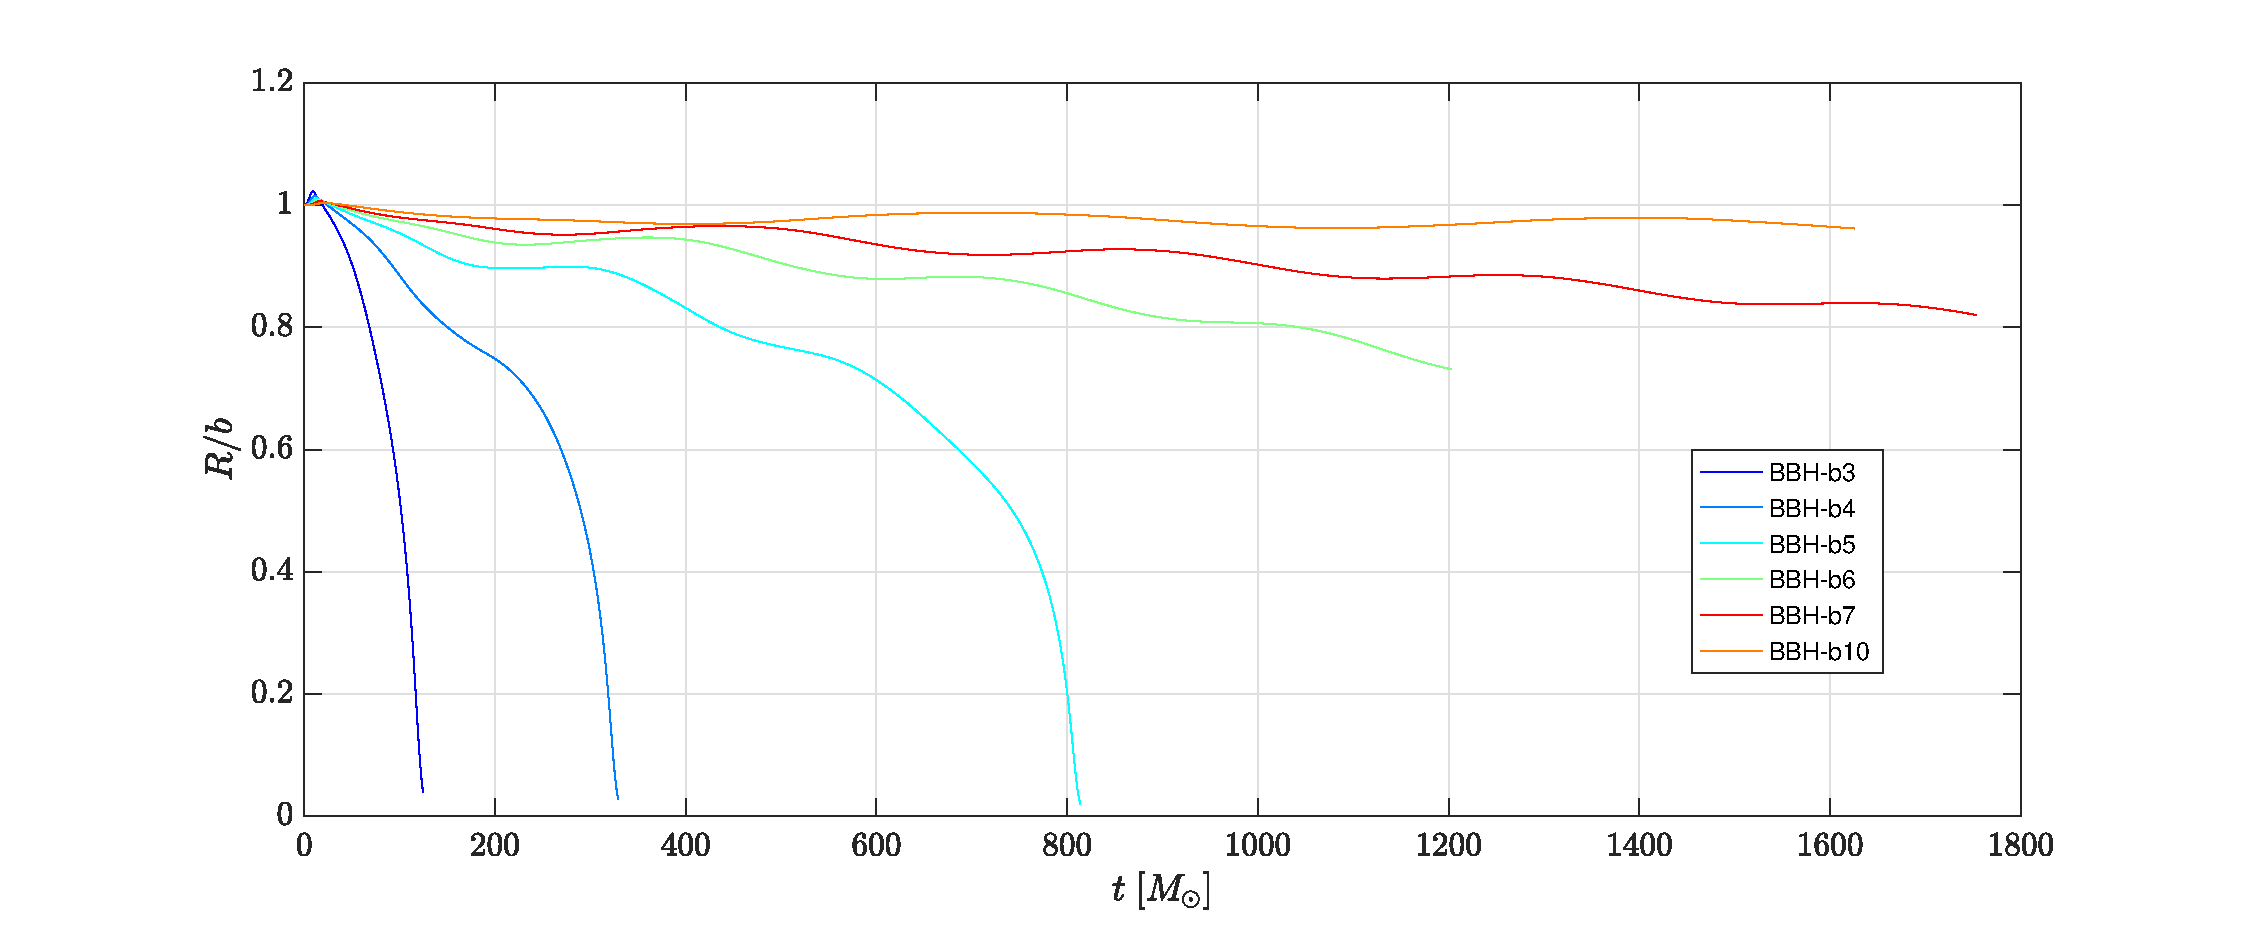
\includegraphics[width=1.1\textwidth]{numerical_evolution/radius_evolution.eps}}
\caption{Time evolution of the distance $R(t)$ between a black hole and the origin of the axes. The values are normalized to the initial separation from the origin $b$. The figure shows oscillation modes especially for BBHs with high $b$.}
\label{radius_evolution}
\end{figure}
%%
%%
%%
%%
\par
We now stufy the gravitational radiation emitted by the different binary sources is extracted following to the procedure described in section(\ref{gw_extraction}).\\
As we have seen in section(\ref{solution_linearized_einstein_eq}) the gravitational radiation scales with the distance from the source as $1/r$.
Therefore, in order to have an order of magnitude of the gravitational wave strain 
\[
h(t) = h_{+} - i h_{\times}
\] 
where $h_{+}$ and $h_{\times}$ are taken from equations(\ref{h_+_numerical}) and (\ref{h_x_numerical}), we multiply $h(t)$ by the distance at which it is was measured and we divide it by a typical cosmological distance of binary sources $r=100 \, \mega \text{pc} \approx 3.1 \times 10^{19} \, \kilo \meter$.
In addition, the units of time will be expressed in millisecond in order to easily compare the frequency of the signals with the sensitivities of the gravitational wave detetctors.



%%
%%
%%
%%
\begin{figure}
\centering
    \textbf{Gravitational waves emitted by BBH}\par\medskip
\centering
\subfloat[][$b=3 \, M_{\odot}$.]
   {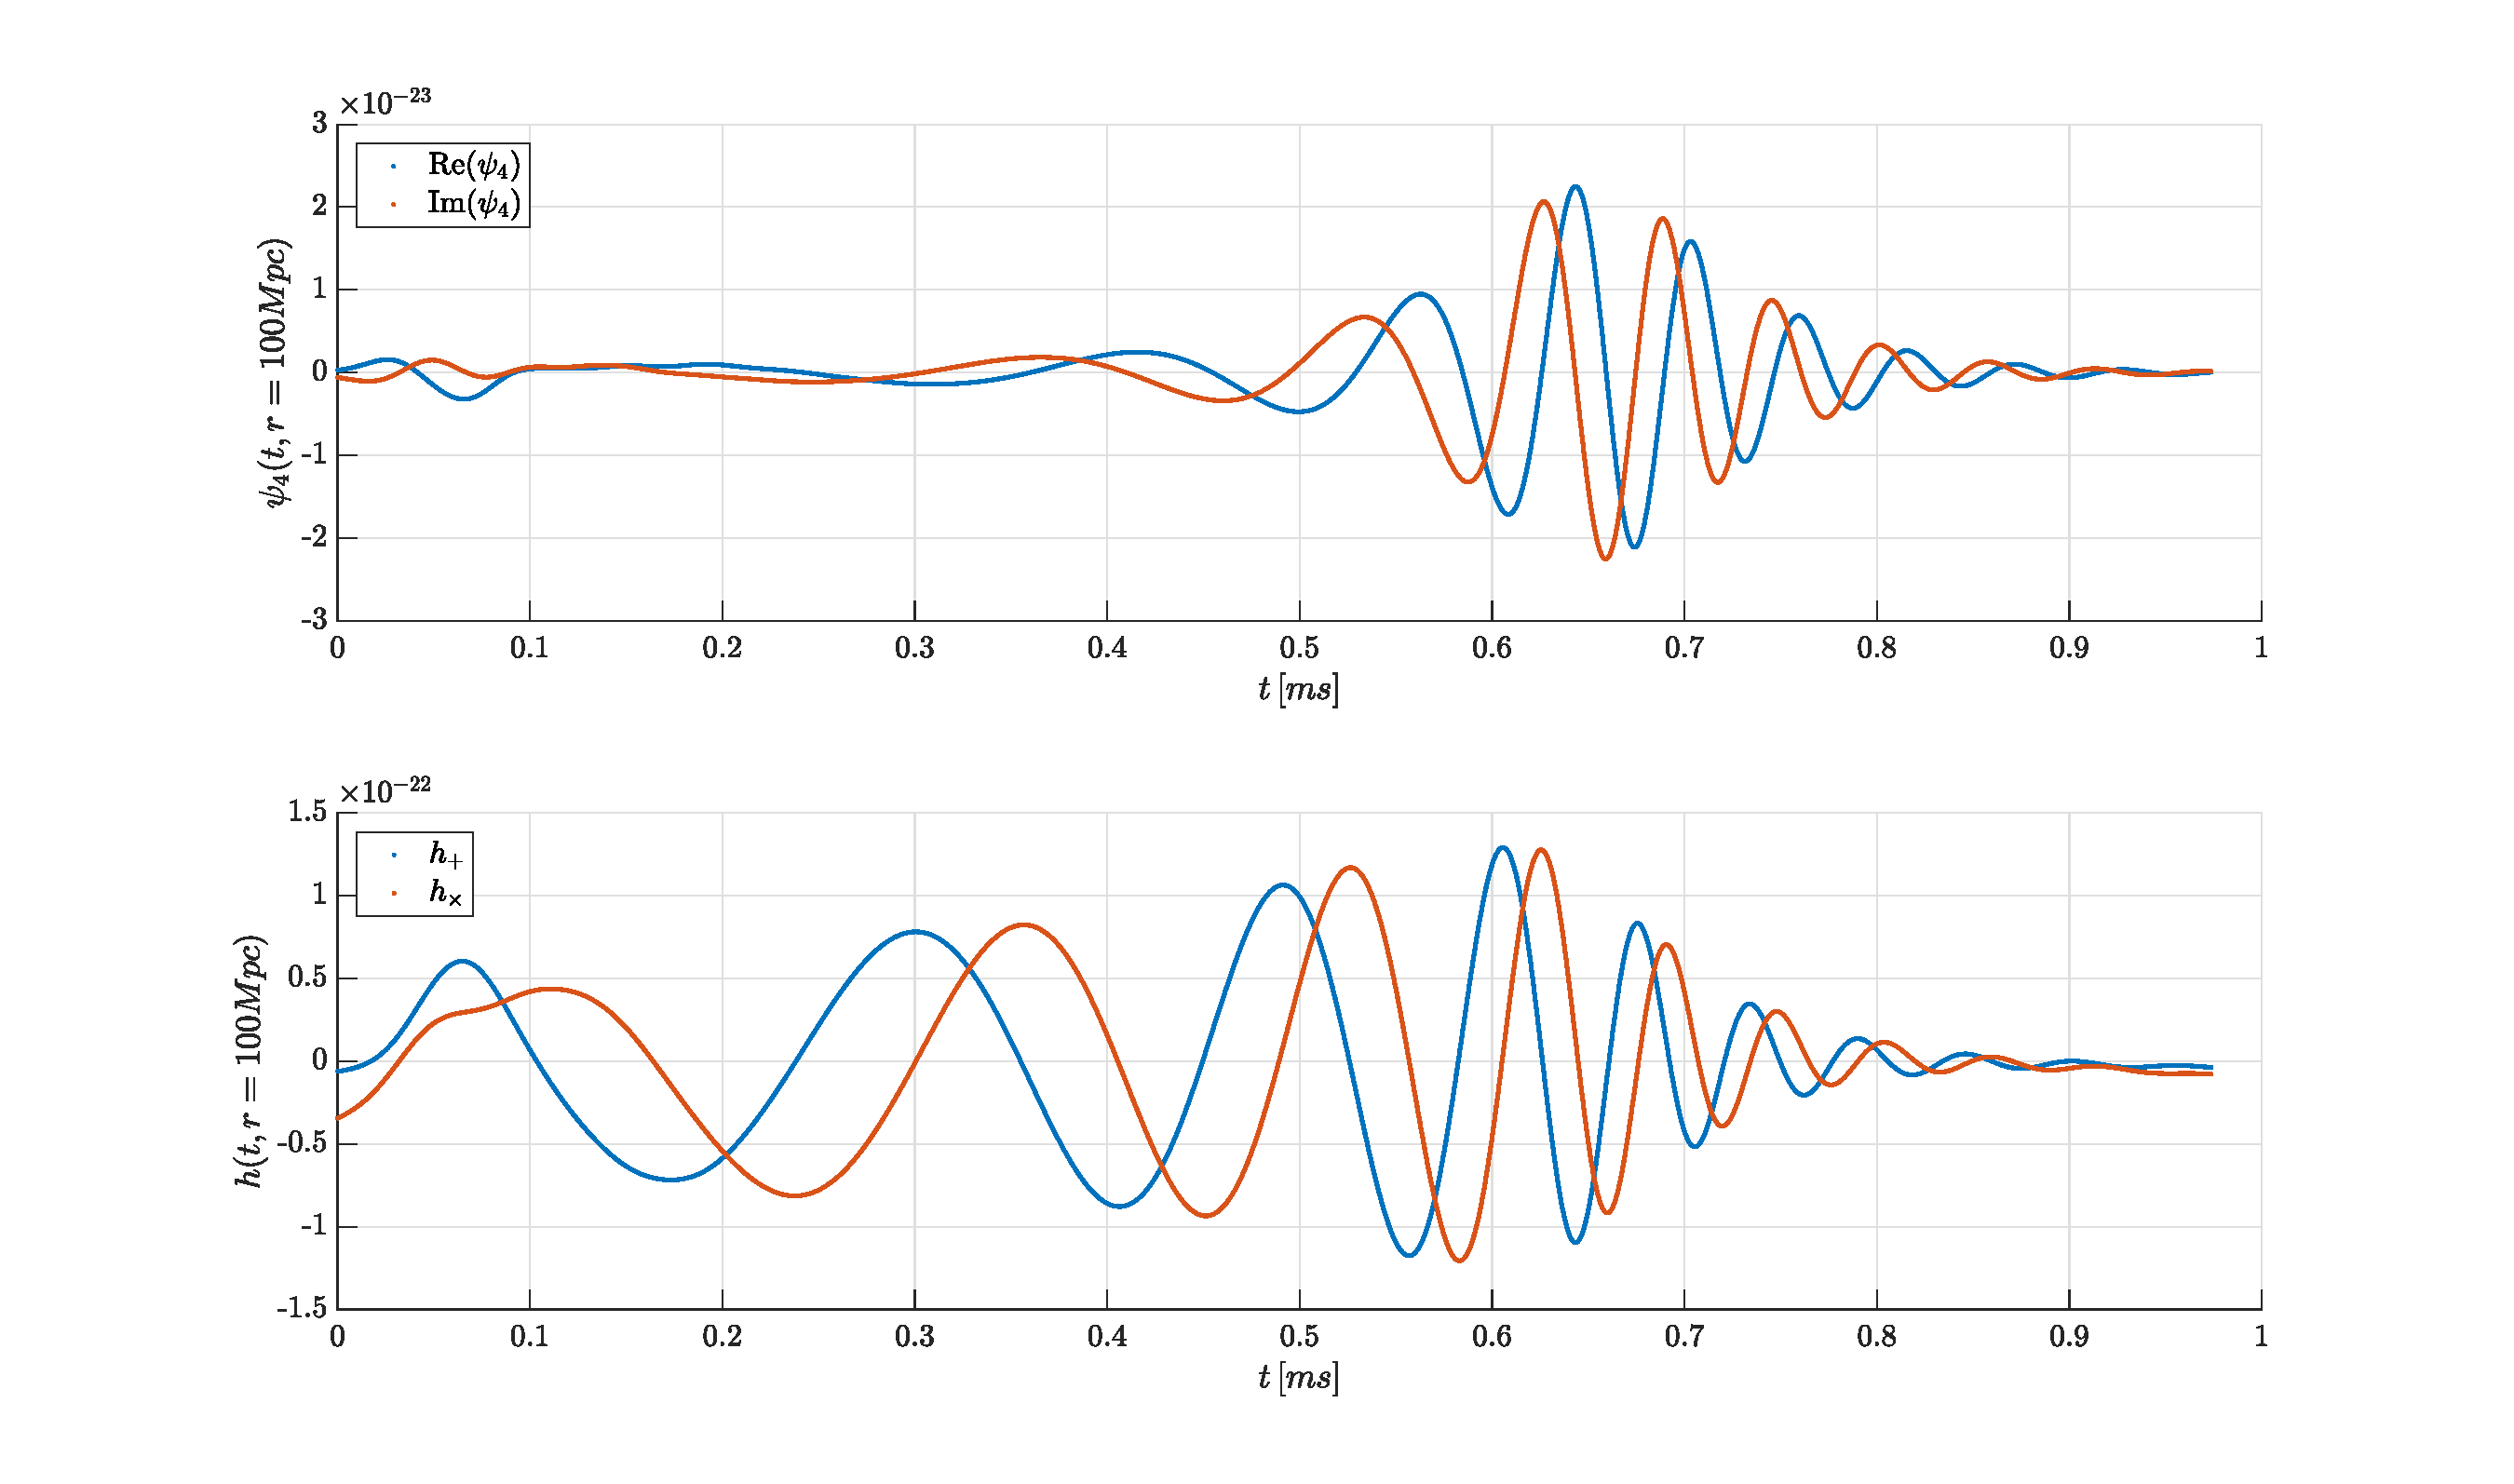
\includegraphics[width=0.9\textwidth]{numerical_evolution/gw_b3.eps}
   \label{gw_b3}} \quad
   \subfloat[][ $b=4 \, M_{\odot}$.]
   {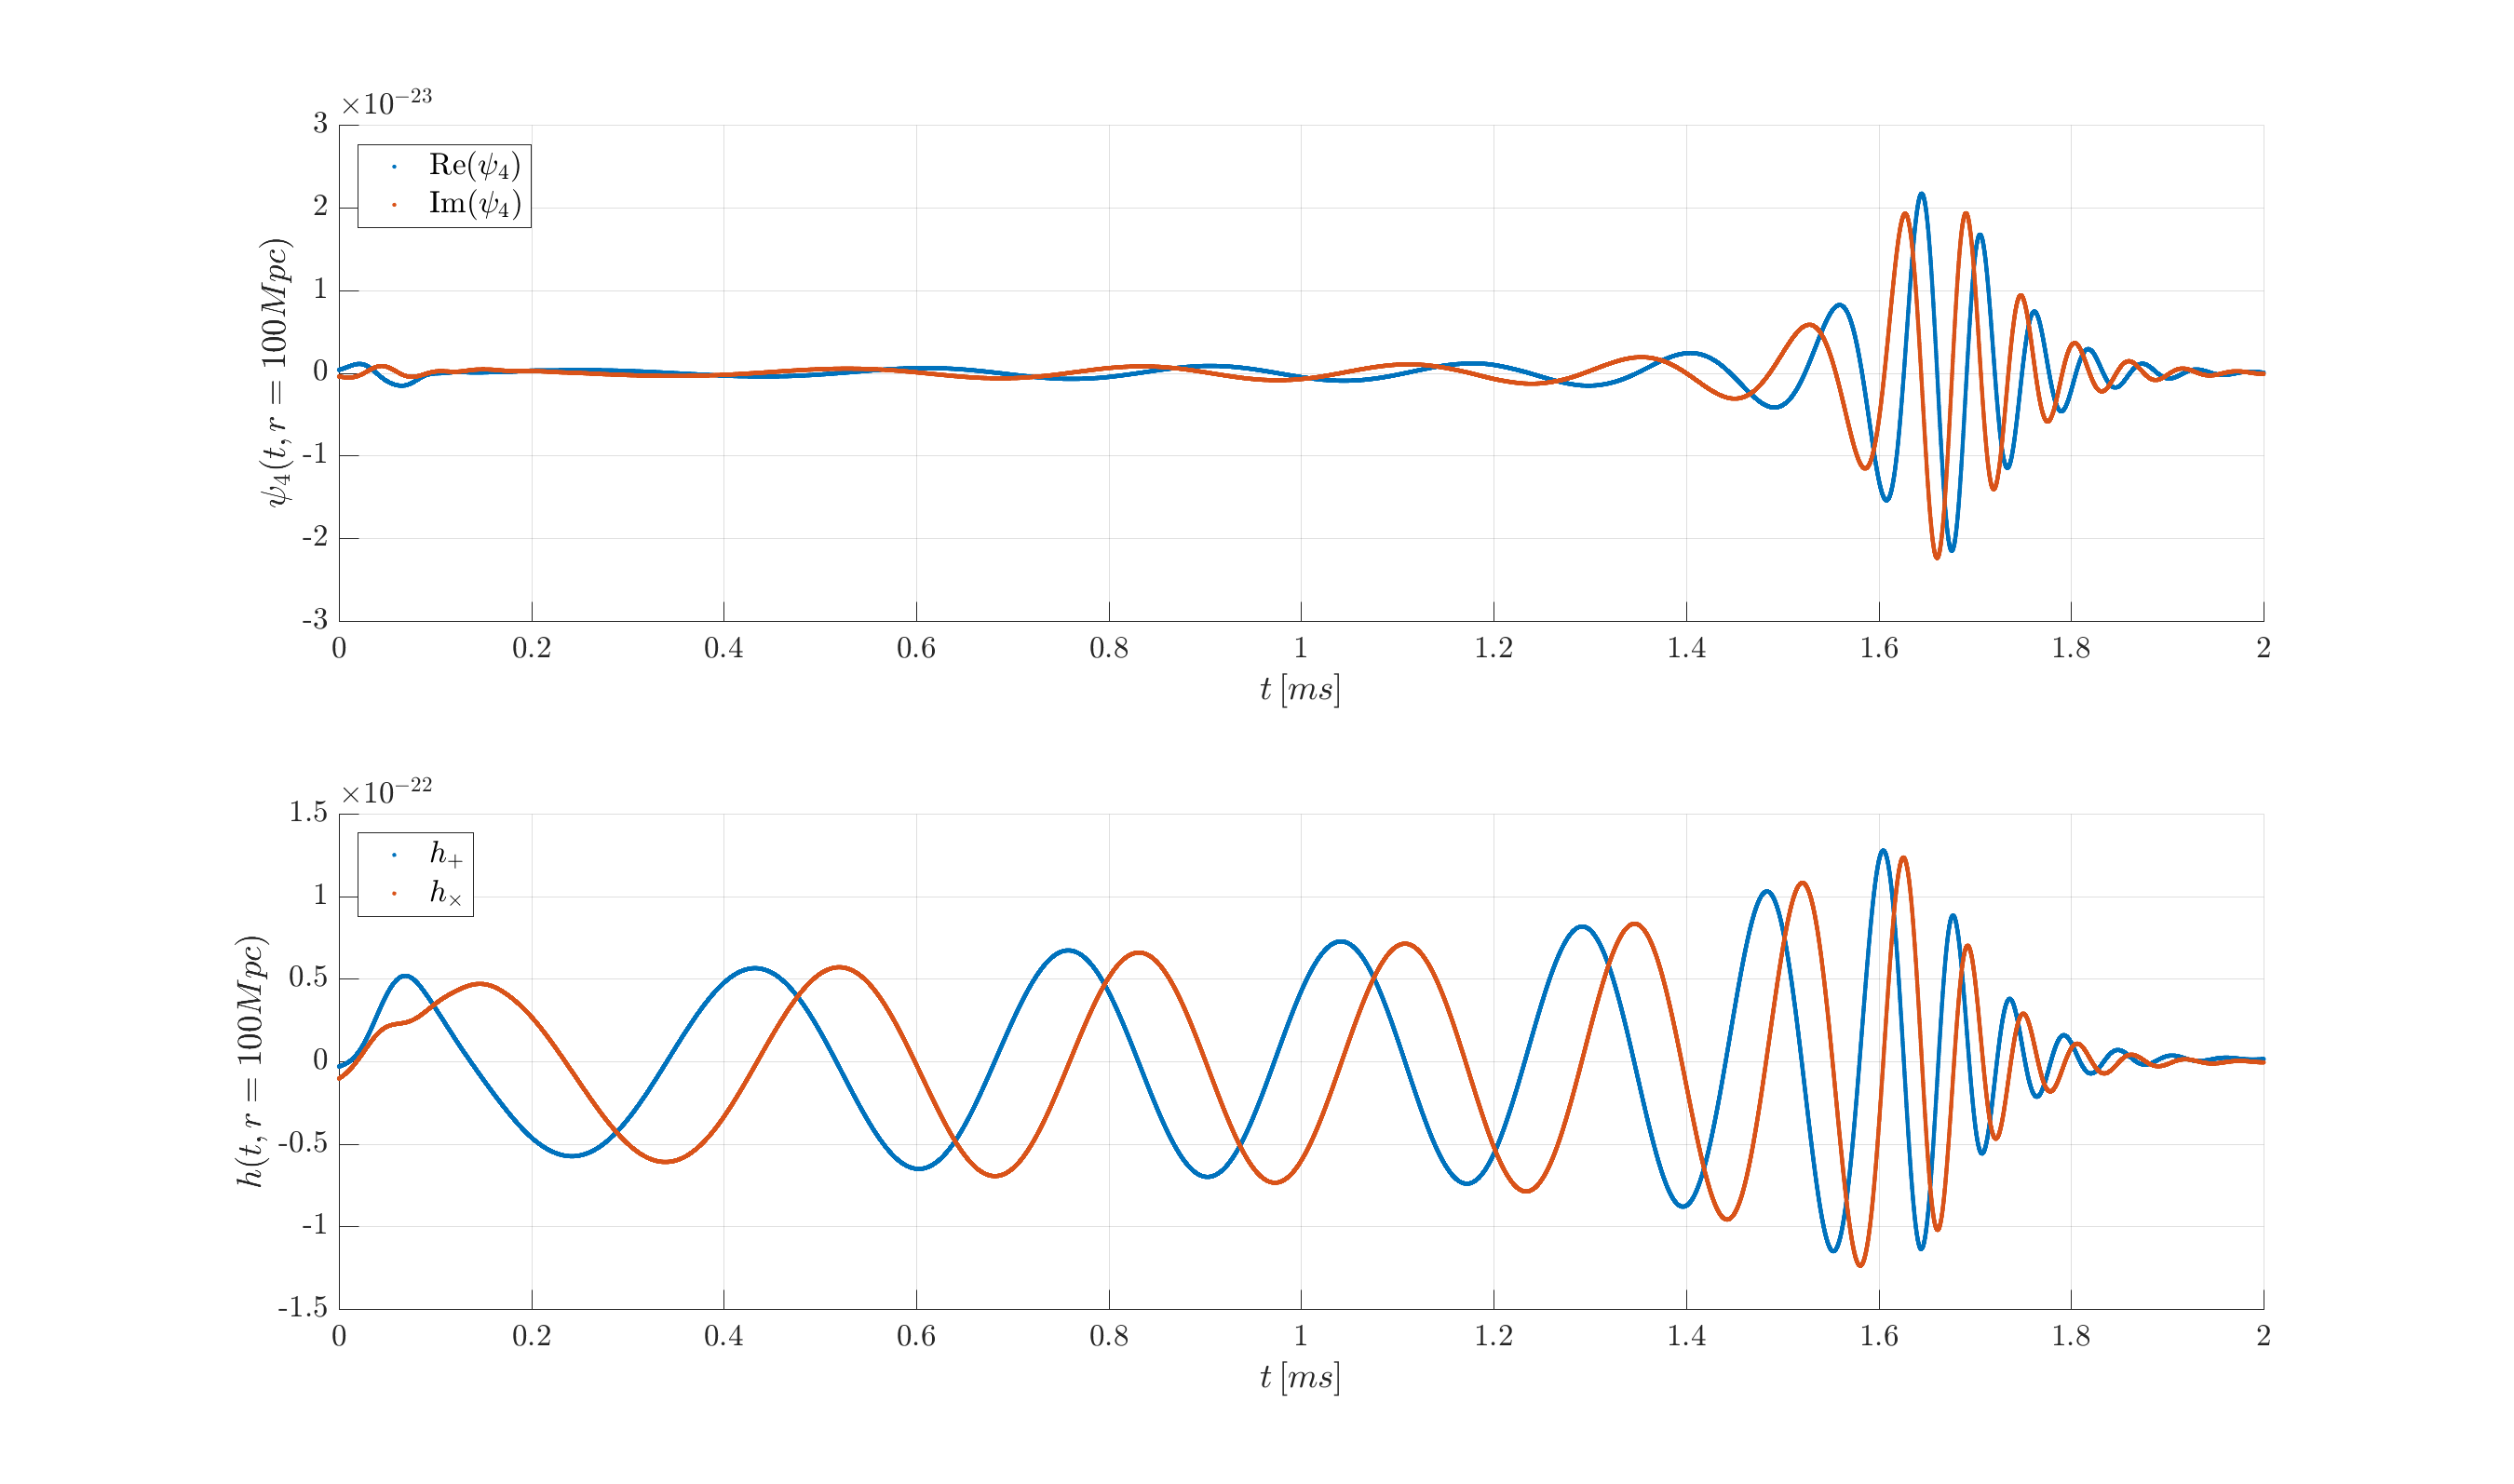
\includegraphics[width=0.9\textwidth]{numerical_evolution/gw_b4.eps}
   \label{gw_b4}} \quad
   \caption{.}
\label{}
\end{figure}
   
   
   \begin{figure}
\centering
    \textbf{Gravitational waves emitted by BBH}\par\medskip
\centering
\subfloat[][$b=5 \, M_{\odot}$.]
   {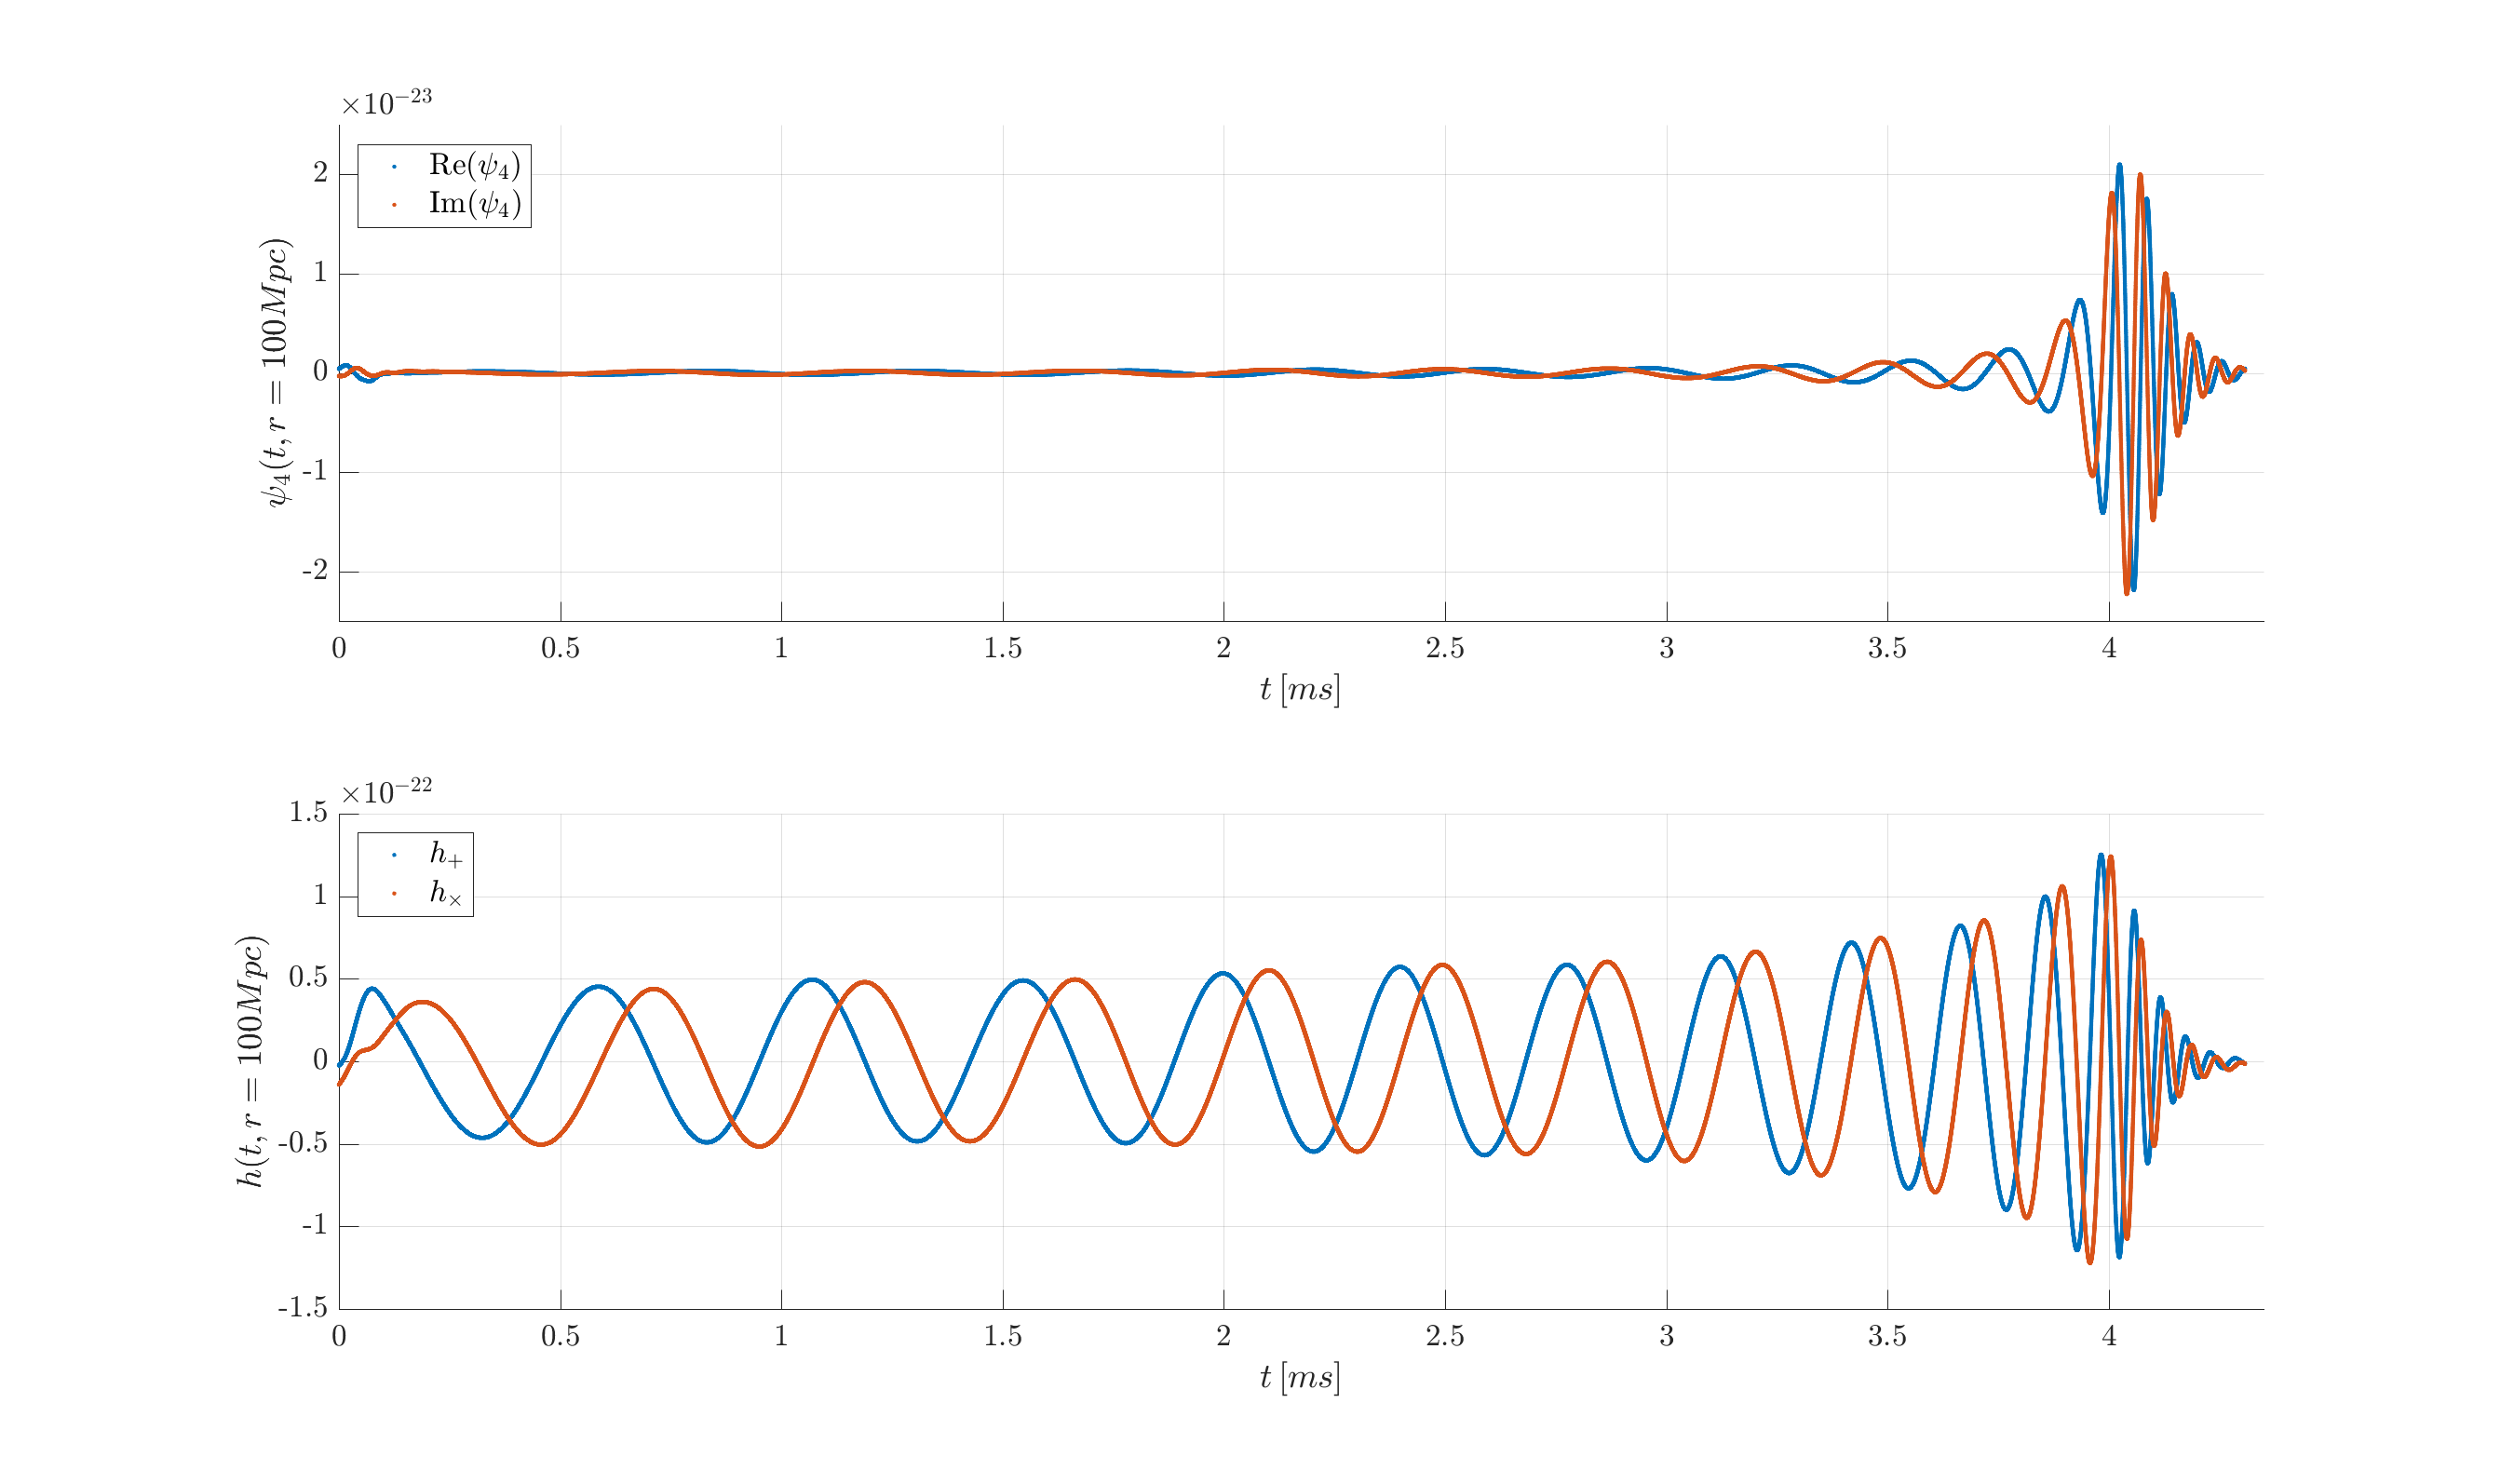
\includegraphics[width=0.9\textwidth]{numerical_evolution/gw_b5.eps}
   \label{gw_b5}}
   \\
\subfloat[][ $b=6 \, M_{\odot}$.]
   {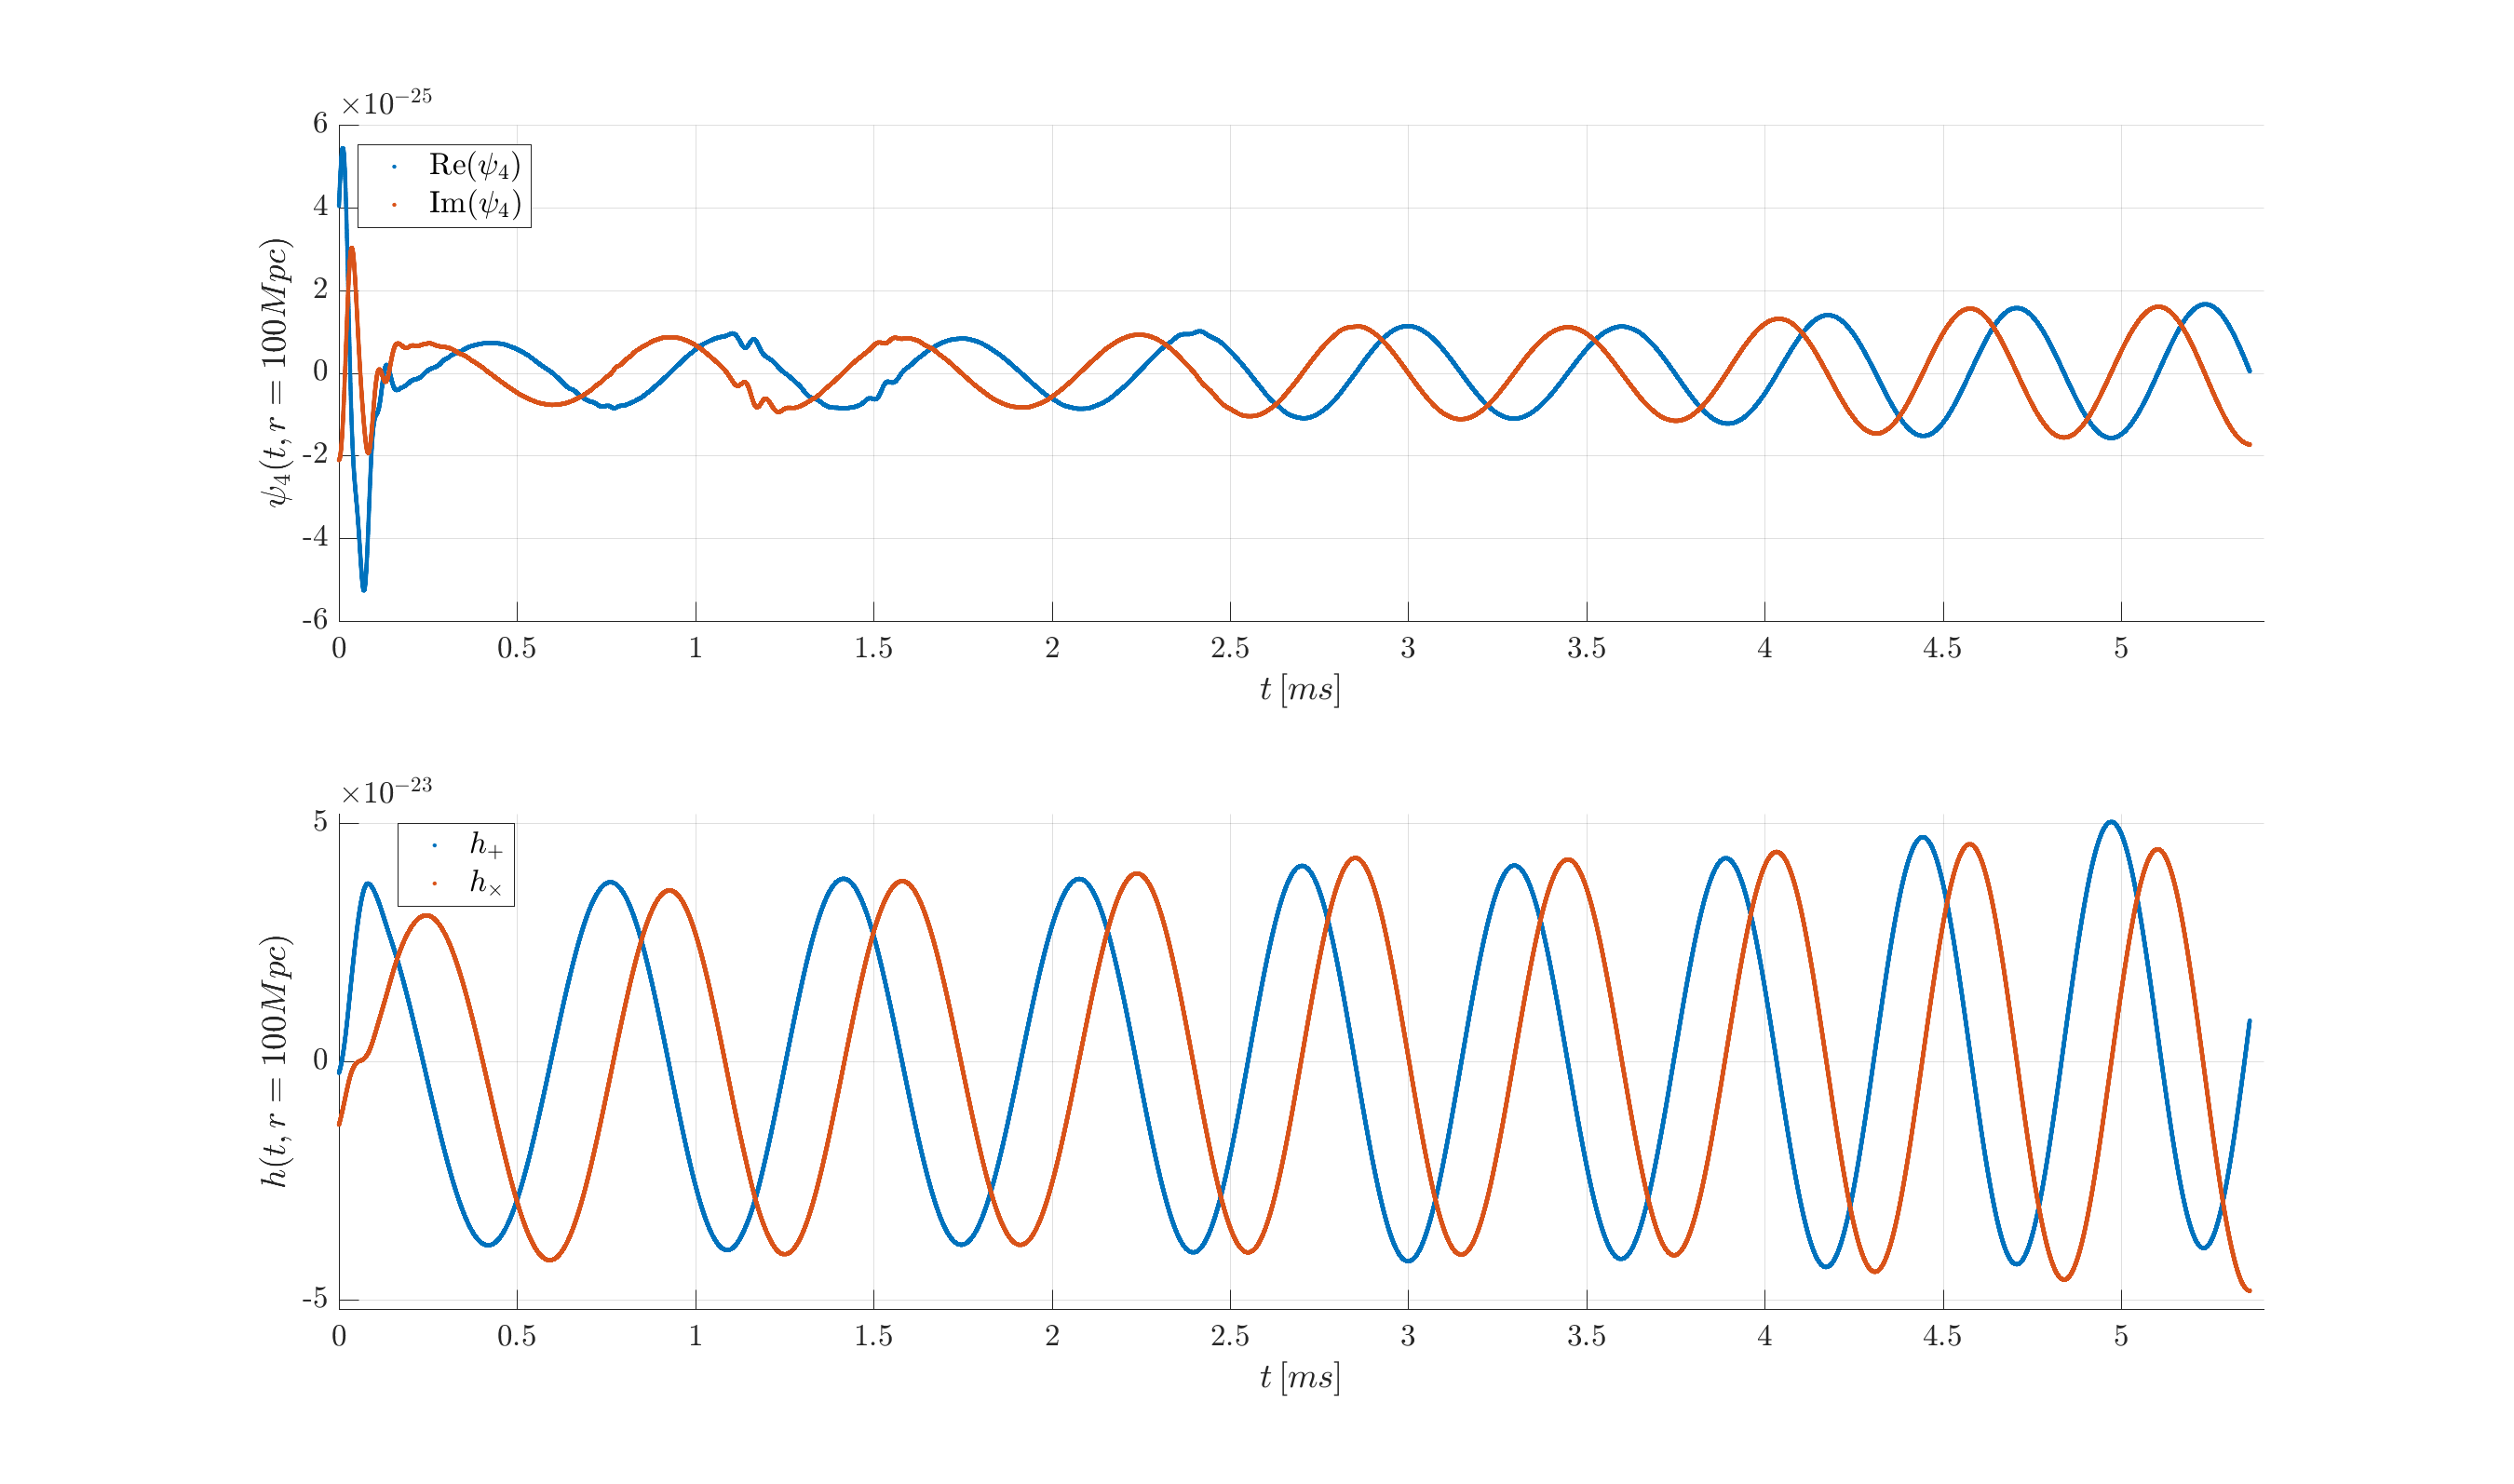
\includegraphics[width=0.9\textwidth]{numerical_evolution/gw_b6.eps}
   \label{gw_b6}} 
   \label{}
\end{figure}
   \begin{figure}
\centering
    \textbf{Gravitational waves emitted by BBH}\par\medskip
\centering
\subfloat[][ $b=7 \, M_{\odot}$.]
   {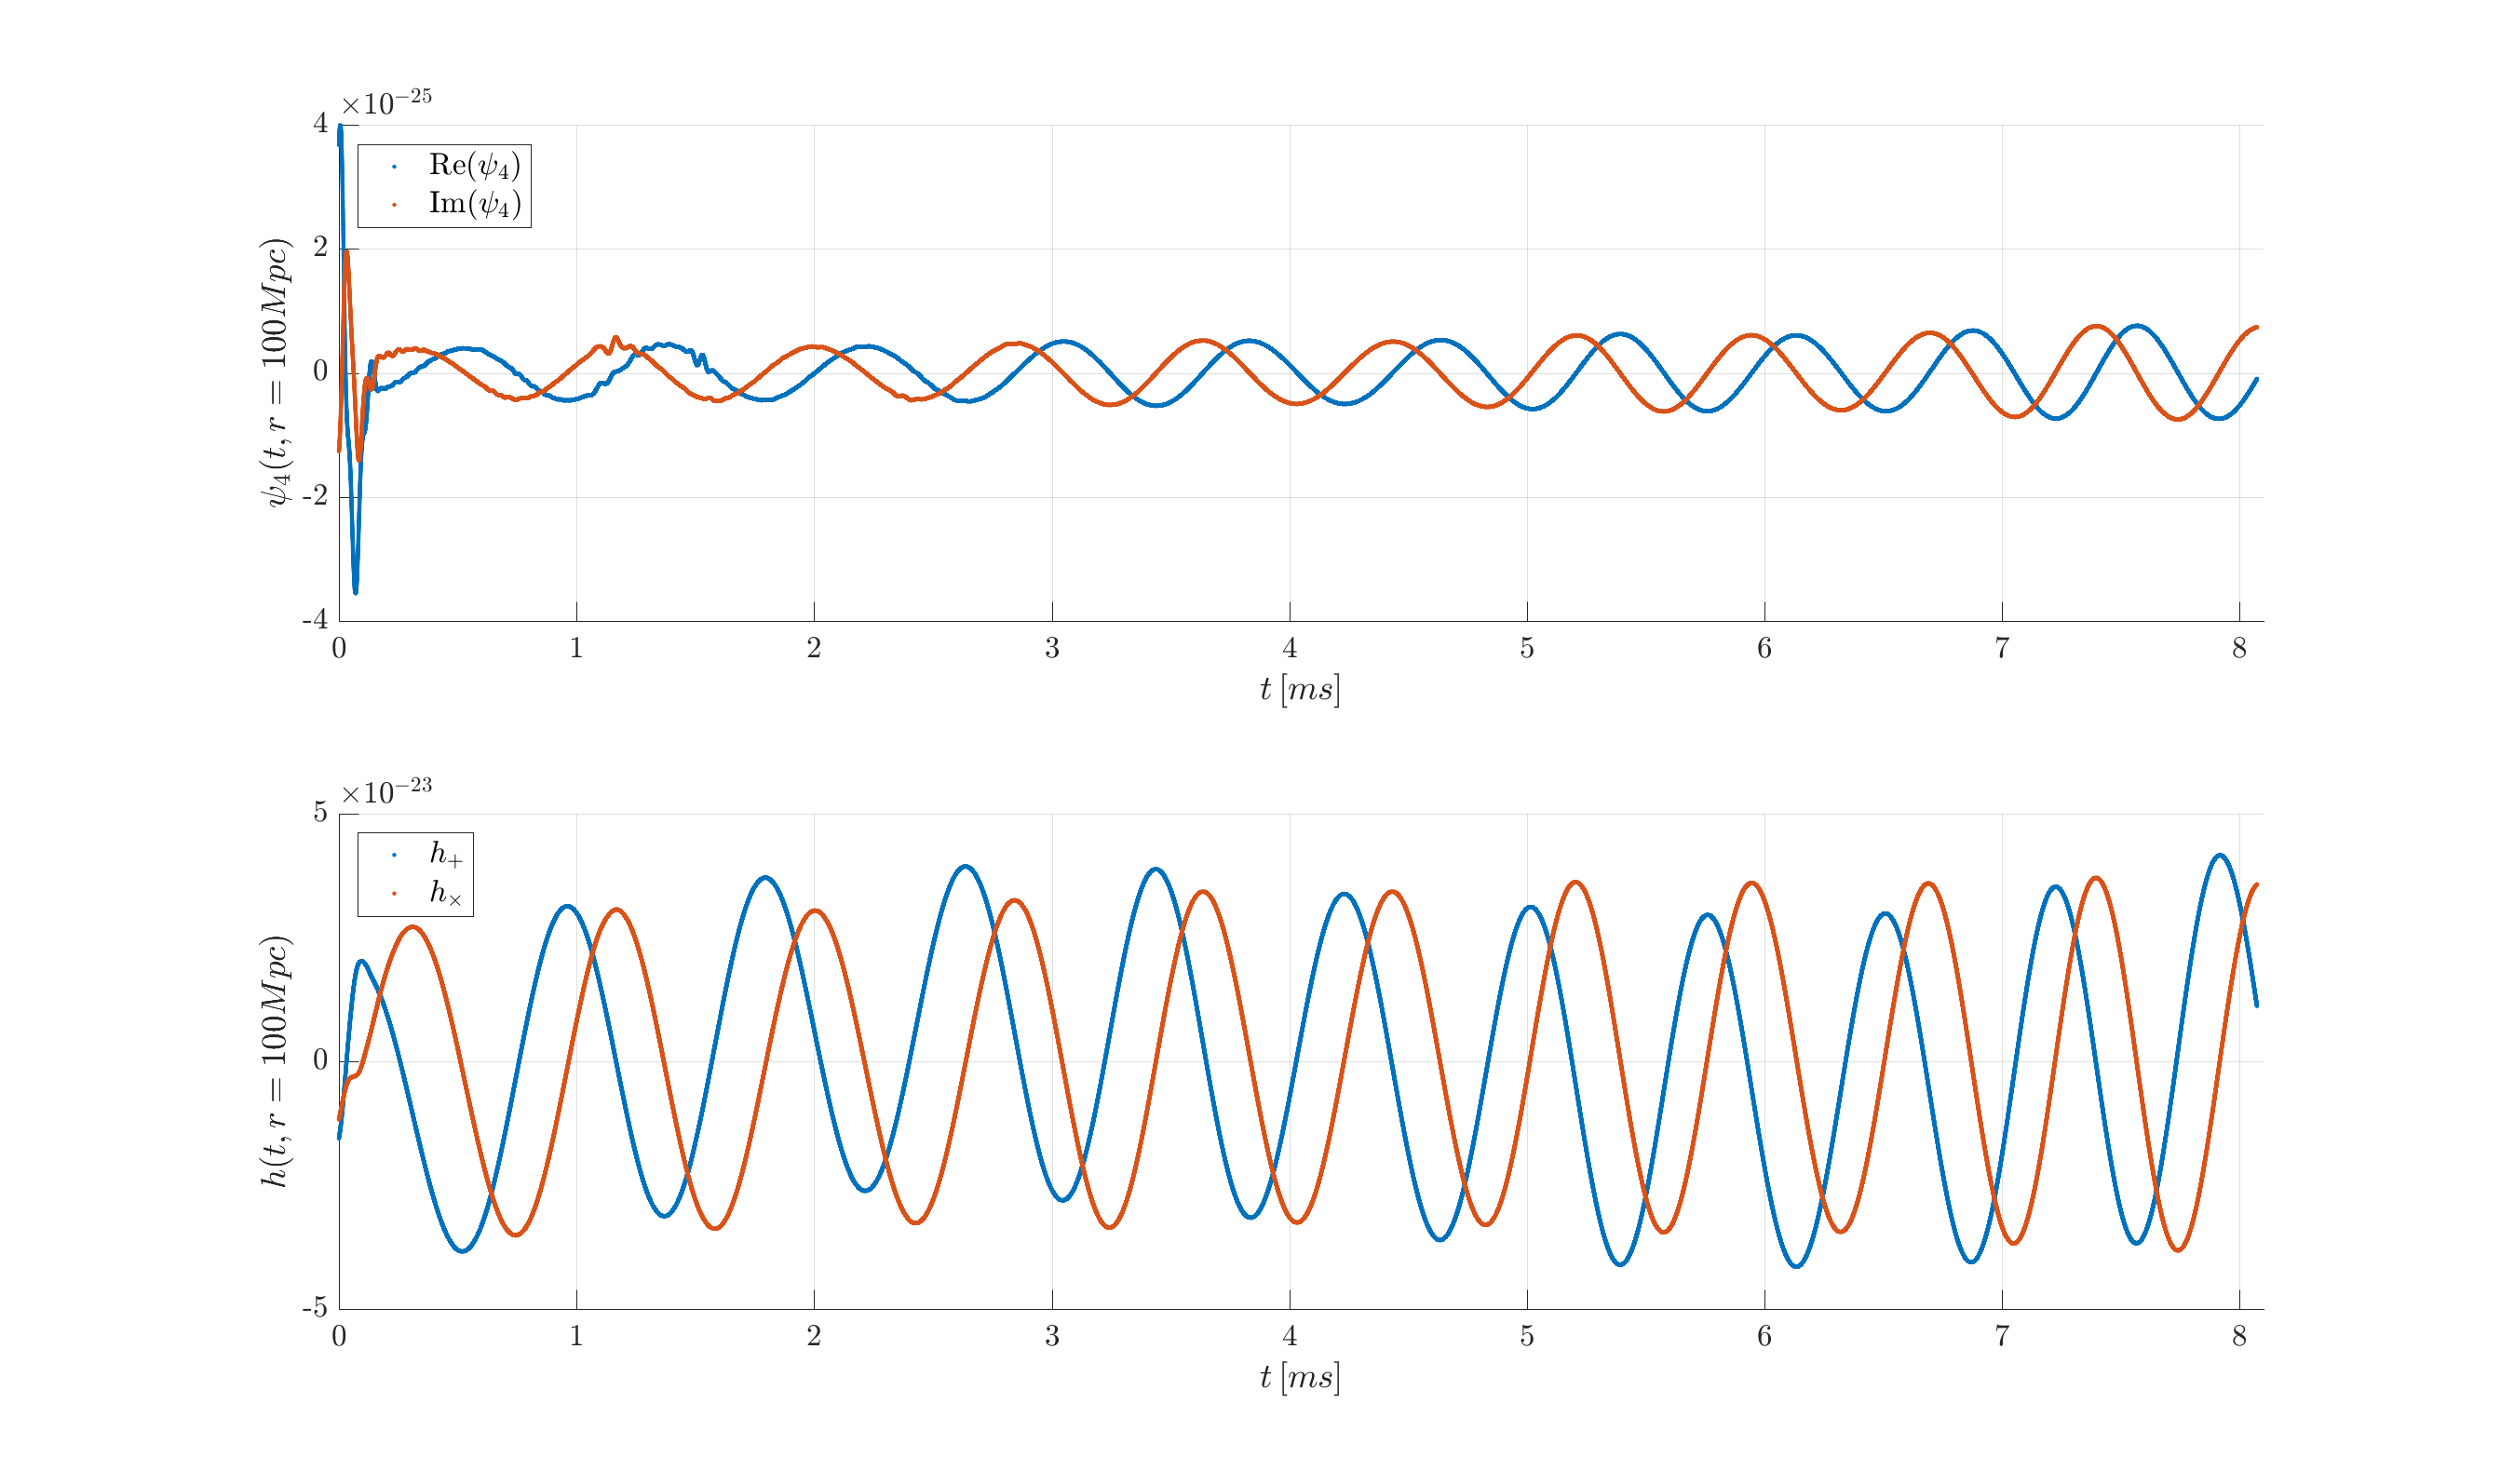
\includegraphics[width=0.9\textwidth]{numerical_evolution/gw_b7.eps}
   \label{gw_b7}} \quad
\subfloat[][ $b=10 \, M_{\odot}$.]
   {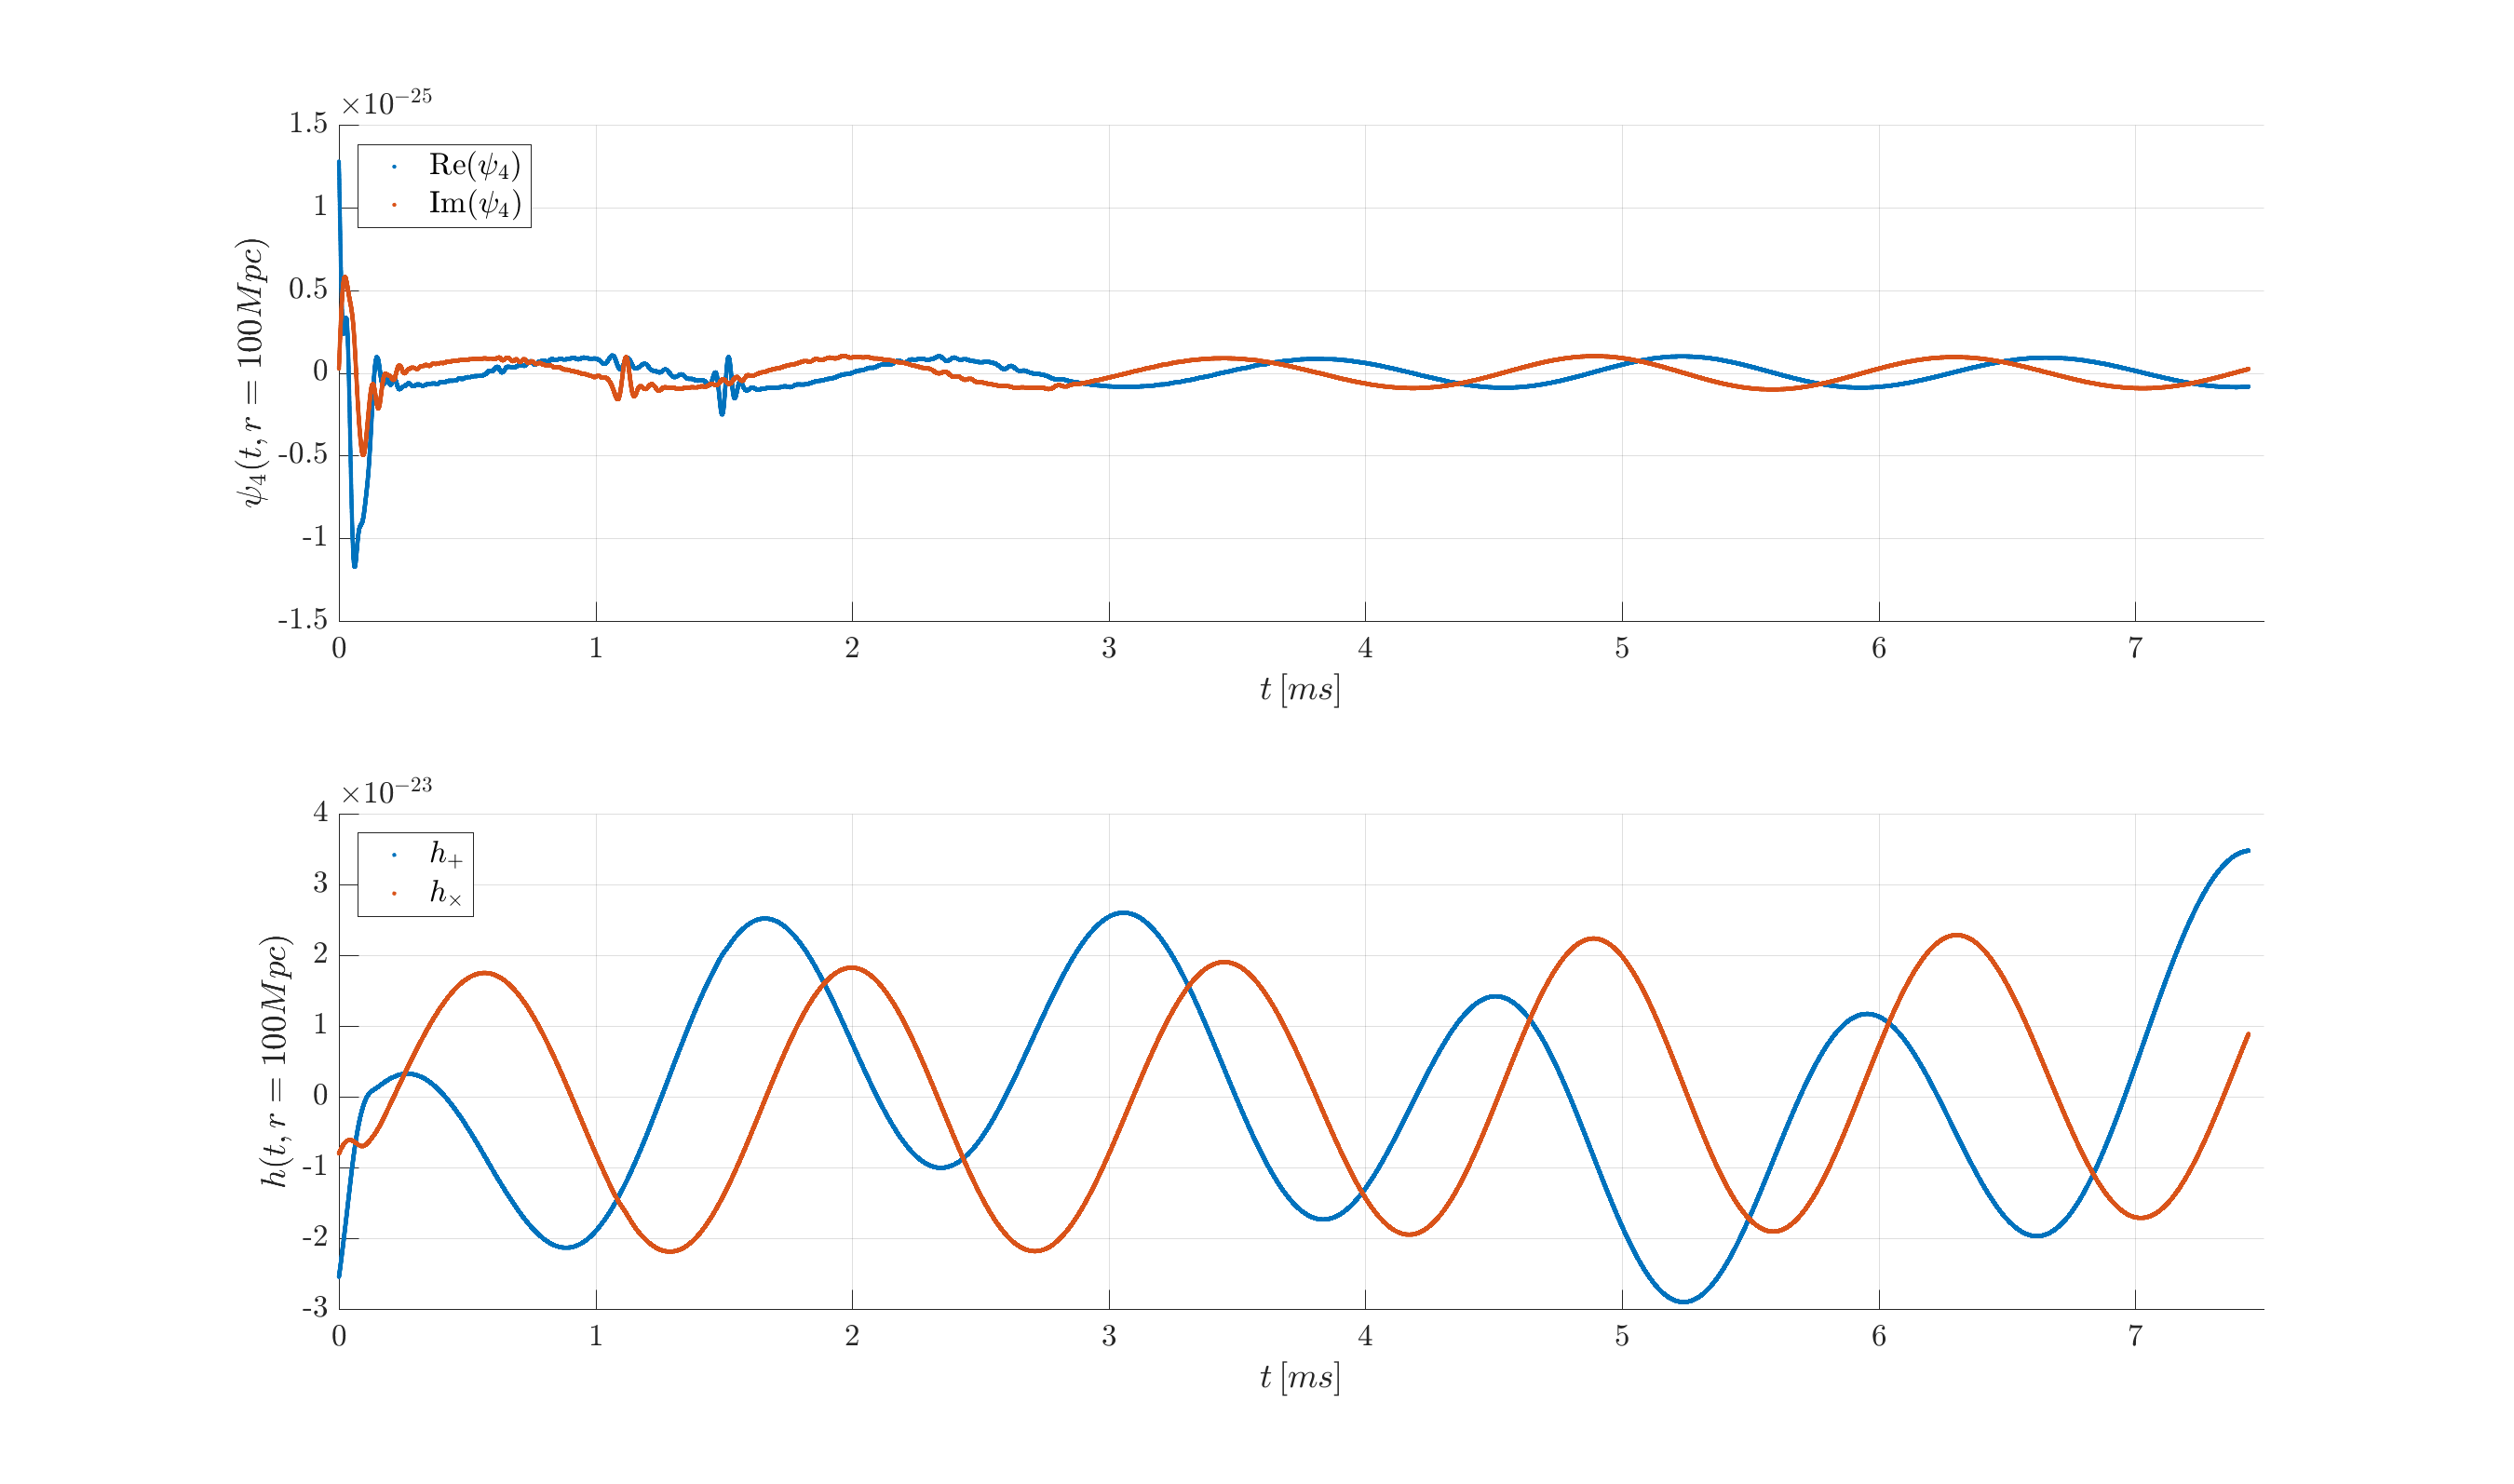
\includegraphics[width=0.9\textwidth]{numerical_evolution/gw_b10.eps}
   \label{gw_b10}} \quad
 \\
\caption{.}
\label{}
\end{figure}
%%
%%
%%
%%


\subsection{Binary Neutron Star}

\clearpage
\section{Conclusions}
Using the weak field linearized equation, the Einstein's field equation in vacuum reduces to a tensorial form of the wave equation (\ref{wave_equation}).
This gravitational wave equation tells us that the metric perturbation behaves as a wave and it travels at the speed of light.
So, the metric perturbation is nothig but a propagating warpage of spacetime, that we call gravitational wave.\\
Using the transverse traceless gaugue, we saw that the polarizations states of the gravitational radiation are only two: $h_{+}$ and $h_{\times}$.
The two polarization modes are directly related to the way they stretch and squeeze spacetime and, therefore, they can change the proper distance between free falling particles according in the shape of $+$ or $\times$.
Such effect can be exploited to detect gravitational waves using interferometers.\\
We analyzed the nature of gravitational wave  and we found out that it has quadrupolar nature and the GW amplitude scales as $1/r$.
We derived the quadrupole formula stressing the importance of the approximations and we applied it to a slowly moving binary system.
The main result of such example told us that the gravitational wave radiation has a frequency that is twice the orbital angular frequency.\\
Subsequently we studied the simualtions of two compact binaries, and through a Fourier analysis we confirmed that the angular frequency of the gravitational waves of BBH and BNS is twice the orbital angular frequency.\\
The orbital angular frequency is almost constant for the first part of the inspiralling phase, and therefore, in this time range it is possible to recognize a sinusoidal behavior of the gravitational wave similiar to the quadrupole formula approximation.
However, the binary system looses energy in the emission of gravitational waves and, therefore, the radius of the binary system decreases. 
As the radius decreases, the orbital angular frequency increases, and therefore, the angular frequency of the gravitational wave does as well. 
During the evolution the aplitude of the GW increases until it reaches the maximum value before the merger.
Both BBH and BNS show similiar gravitational singnals during the inspiralling phase.\\
For a binary black hole, the gravitational wave signal is damped after the merger, whereas for the considered binary neutron star, the radiation amplitude slowly decreases.
Furthermore, the bouncing in the gravitational wave amplitude of the BNS denotes that the cores are bouncing off each other.\\
In addition, we tested succesfully the codes provided by the Einstein Toolkit \cite{EinsteinToolkit:web}, and we also tested the quasi-equilibrium initial conditions of \cite{tichy_quasi-equilibrium_2004}.\\
Further researches and more accurate simulations should be done in order to precisely explain the oscillations mode of the orbital angular frequency and of the gravitational strain of BBH-b6, BBH-b7, BBH-b10.\\
By combining the computational power of numerical relativity with the new "eyes" given by the gravitational wave detector, we will be able to understand thoroughly the connections between fascinating objects such black holes and neutron stars and the gravitational waves.







%% APPENDICES
\clearpage
\section*{Acknowledgements}
I wish to acknowledge the help received from some people and organizations during the developing of this project.\\
First and foremost, i must thank my supervisor, prof. Bruno Giacomazzo, who introduced me to the fascinating world of numerical relativity through the Einstein Toolkit. \\
I would also like to acknowledge the computational physics group at the University of Oslo, for providing me the access to the cluster "Smaug". 
Without the compuational power of "Smaug", I would have not run the numerical simulations shown in this work.\\
I would also like to thank Giovanni Pederiva, who constantly taught me many crucial numerical concepts.\\
Finally, I must express my very profound gratitude to my family, my girlfriend and my friends for providing me with unfailing support and continuous encouragement.
This accomplishment would not have been possible without them.\\
Thank you.\\

Lorenzo Speri

%% MAKE BIBLIOGRAPHY
%\bibliographystyle{unsrt}
\clearpage
\printbibliography


%% AND SO WE END
\end{document}

